\documentclass[aspectratio=169]{beamer}

\usetheme{Madrid}

\usepackage[utf8]{inputenc}
\usepackage[T1]{fontenc}
\usepackage[brazil]{babel}
\usepackage{amsmath,amssymb,amsfonts}
\usepackage{graphicx}
\usepackage{tikz}
\usepackage[most]{tcolorbox}
\usepackage{pgfplots}
\pgfplotsset{compat=1.18}
\usetikzlibrary{calc}

%-------------------------------------------------
% Cores padrão
%-------------------------------------------------
\definecolor{myblue}{RGB}{0,86,125}
\definecolor{mycyan}{RGB}{0,183,235}
\definecolor{myred}{RGB}{160,30,30}
\definecolor{mygray}{RGB}{245,247,250}
\definecolor{mydark}{RGB}{20,35,45}

\setbeamercolor{structure}{fg=myblue}
\setbeamercolor{frametitle}{bg=myblue,fg=white}
\setbeamercolor{title}{fg=white}

%-------------------------------------------------
% Boxes padrão
%-------------------------------------------------
\newtcolorbox{mybox}[1]{
colback=mygray,
colframe=myblue,
title=#1,
fonttitle=\bfseries,
arc=3mm,
boxrule=0.8pt
}

\newtcolorbox{eqbox}{
colback=white,
colframe=mycyan,
arc=3mm,
boxrule=0.8pt
}

%-------------------------------------------------
% Figura com placeholder
%-------------------------------------------------
\newcommand{\figplaceholder}[3]{
\begin{center}
\IfFileExists{#1}{
\includegraphics[width=#2\textwidth]{#1}
}{
\fbox{
\begin{minipage}[c][0.28\textheight][c]{#2\textwidth}
\centering
Figura: \texttt{#1}
\end{minipage}
}
}


{\scriptsize #3}
\end{center}
}


\newcommand{\notas}[1]{%
\begin{tikzpicture}[remember picture,overlay]
\node[anchor=south west,
      xshift=3mm,
      yshift=3mm,
      draw,
      rectangle,
      rounded corners=2pt,
      fill=white,
      font=\tiny,
      inner sep=2pt]
at (current page.south west)
{Notas: #1};
\end{tikzpicture}
}
%-------------------------------------------------
% Capa bonita padrão
%-------------------------------------------------
\newcommand{\beautifulcover}{
{
\setbeamertemplate{navigation symbols}{}
\begin{frame}[plain]
\begin{tikzpicture}[remember picture,overlay]
\fill[mydark] (current page.south west) rectangle (current page.north east);

\fill[myblue!70] 
([xshift=-2.5cm,yshift=1.5cm]current page.south west) circle (4.5cm);

\fill[mycyan!45] 
([xshift=2.5cm,yshift=-1.0cm]current page.north east) circle (4.2cm);

\fill[white,opacity=0.05]
([xshift=0.0cm,yshift=0.0cm]current page.center) circle (7.5cm);

\node[align=center,text=white] at (current page.center) {
{\Huge\bfseries Multipolos Elétricos}\\[0.35cm]
{\Large Capítulo 4}\\[0.55cm]
{\large Eletrodinâmica Clássica}
};

\node[align=center,text=white!75] at ([yshift=-3.1cm]current page.center) {
Prof. Dr. Rafael Camargo Rodrigues de Lima
};
\end{tikzpicture}
\end{frame}
}
}

\begin{document}

\beautifulcover

\begin{frame}[plain]

\begin{tikzpicture}[remember picture,overlay]
\node at (current page.center) {
    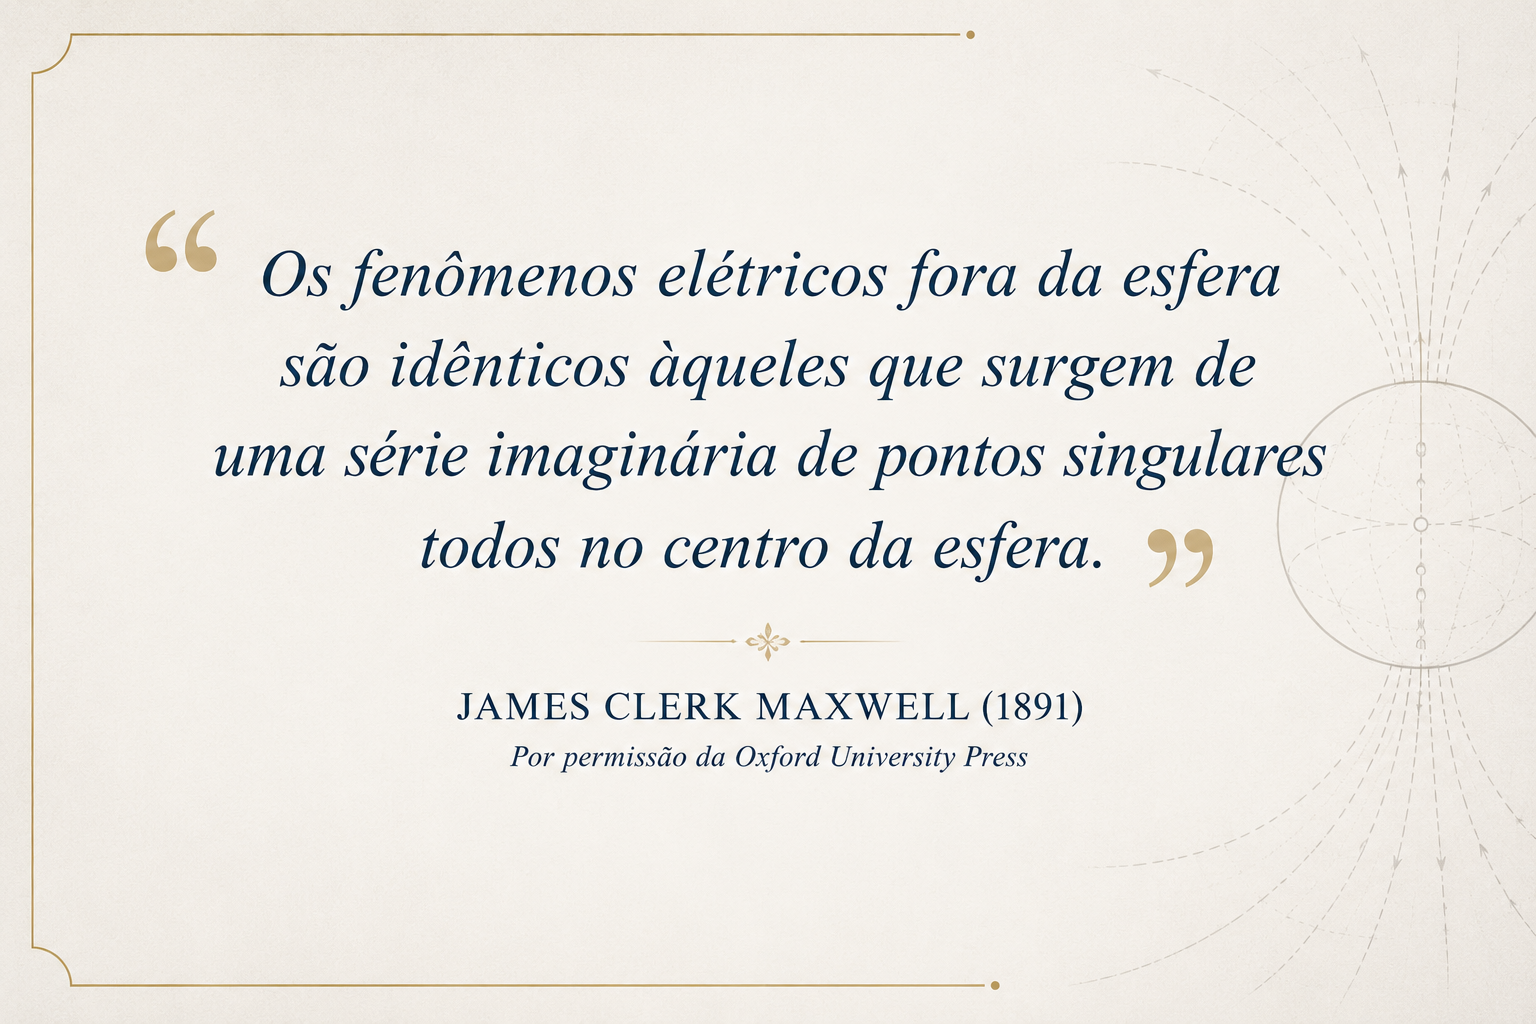
\includegraphics[
        width=\paperwidth,
        height=\paperheight
    ]{ChatGPT Image 12 de mai. de 2026, 08_41_07.png}
};
\end{tikzpicture}

\end{frame}

%====================================================
\begin{frame}{Motivação para a Expansão Multipolar}

\begin{mybox}{Escalas físicas muito diferentes}

Em muitos problemas físicos, o observador está muito distante da distribuição de cargas.

\medskip

Exemplos:

\begin{itemize}

\item partículas subatômicas;

\item átomos e moléculas;

\item distribuições biológicas de carga;

\item núcleos atômicos observados pelos elétrons.

\end{itemize}

\end{mybox}

\end{frame}

\begin{frame}
\begin{alertblock}{Ideia central}

Se estamos muito longe da fonte, não precisamos conhecer todos os detalhes microscópicos da distribuição de cargas.

Podemos construir uma aproximação sistemática do potencial eletrostático válida para grandes distâncias.

\end{alertblock}

\begin{mybox}{Distribuição localizada}

Chamamos a distribuição de cargas de \textbf{localizada} quando ela ocupa apenas uma região finita do espaço, de tamanho típico \(R\).

\end{mybox}



\end{frame}


%====================================================


%-------------------------------------------------
\begin{frame}{Ideia central do capítulo}

\begin{mybox}{Problema físico}
Queremos calcular o potencial eletrostático produzido por uma distribuição localizada de carga.
\end{mybox}

\begin{eqbox}
\begin{equation}
\varphi(\mathbf r)
=
\frac{1}{4\pi\epsilon_0}
\int
\frac{\rho(\mathbf r')}{|\mathbf r-\mathbf r'|}
\,d^3r' .
\tag{4.1}
\label{eq:potencial_coulomb}
\end{equation}
\end{eqbox}

\begin{alertblock}{Consequência física}

O potencial pode ser escrito como uma soma de termos sucessivos:

\[
\text{monopolo}
\rightarrow
\text{dipolo}
\rightarrow
\text{quadrupolo}
\rightarrow \cdots
\]

Cada termo carrega informações diferentes sobre a geometria da fonte.

\end{alertblock}

\end{frame}

\begin{frame}

\begin{mybox}{Ideia da expansão multipolar}
Se a carga está concentrada numa região de tamanho \(R\) e o observador está longe,
\[
r \gg R,
\]
então podemos aproximar o potencial por termos sucessivos.
\end{mybox}

\end{frame}

%-------------------------------------------------
\begin{frame}{Geometria do problema}

\figplaceholder{4p1.png}{0.5}{
Figura 4.1: distribuição localizada de carga dentro de uma esfera de raio \(R\), com ponto de observação em \(r\gg R\).
}

\begin{mybox}{Interpretação}
O vetor \(\mathbf r'\) localiza os elementos de carga dentro da distribuição, enquanto \(\mathbf r\) aponta da origem até o observador.
\end{mybox}

\end{frame}

%-------------------------------------------------
\begin{frame}{Por que podemos expandir?}

\begin{mybox}{Hipótese de campo distante}
Como toda a carga está dentro de uma esfera de raio \(R\), temos
\[
|\mathbf r'| \leq R.
\]
Para um observador distante,
\[
|\mathbf r'| \ll |\mathbf r|.
\]
\end{mybox}

\begin{eqbox}
\begin{equation}
\frac{1}{|\mathbf r-\mathbf r'|}
=
\frac{1}{r}
-
\mathbf r'\cdot \nabla \frac{1}{r}
+
\frac{1}{2}
r'_i r'_j
\nabla_i\nabla_j
\frac{1}{r}
+\cdots .
\tag{4.2}
\label{eq:taylor_multipolar}
\end{equation}
\end{eqbox}
\notas{pag. 1-5}
\end{frame}

%-------------------------------------------------
\begin{frame}{Primeiro passo: calcular o gradiente}

\begin{mybox}{Gradiente de \(1/r\)}
Como
\[
r=\sqrt{x^2+y^2+z^2},
\]
temos
\[
\frac{\partial r}{\partial x_i}
=
\frac{x_i}{r}.
\]
\end{mybox}

\begin{eqbox}
\begin{equation}
\nabla_i\frac{1}{r}
=
-\frac{1}{r^2}\frac{\partial r}{\partial x_i}
=
-\frac{x_i}{r^3}.
\label{eq:gradiente_um_sobre_r}
\end{equation}
\end{eqbox}

\end{frame}

\begin{frame}

Portanto,

\begin{eqbox}
\begin{equation}
\nabla\frac{1}{r}
=
-\frac{\mathbf r}{r^3}.
\label{eq:gradiente_vetorial}
\end{equation}
\end{eqbox}

\end{frame}

%-------------------------------------------------
\begin{frame}{Segundo passo: o termo dipolar}

\begin{eqbox}
\begin{equation}
-\mathbf r'\cdot \nabla\frac{1}{r}
=
-\mathbf r'\cdot
\left(
-\frac{\mathbf r}{r^3}
\right)
=
\frac{\mathbf r'\cdot \mathbf r}{r^3}.
\label{eq:termo_dipolar_kernel}
\end{equation}
\end{eqbox}

\begin{mybox}{Resultado até primeira ordem}
\[
\frac{1}{|\mathbf r-\mathbf r'|}
=
\frac{1}{r}
+
\frac{\mathbf r'\cdot\mathbf r}{r^3}
+\cdots .
\]
\end{mybox}

\end{frame}

%-------------------------------------------------
\begin{frame}{Substituindo no potencial}

Substituímos a expansão na integral de Coulomb:

\begin{eqbox}
\begin{equation}
\varphi(\mathbf r)
=
\frac{1}{4\pi\epsilon_0}
\int d^3r'\,\rho(\mathbf r')
\left[
\frac{1}{r}
+
\frac{\mathbf r'\cdot\mathbf r}{r^3}
+\cdots
\right].
\label{eq:potencial_expandido_inicial}
\end{equation}
\end{eqbox}

Separando os termos:

\begin{eqbox}
\begin{equation}
\varphi(\mathbf r)
=
\frac{1}{4\pi\epsilon_0}
\left[
\frac{1}{r}
\int \rho(\mathbf r')\,d^3r'
+
\frac{\mathbf r}{r^3}\cdot
\int \mathbf r'\rho(\mathbf r')\,d^3r'
+\cdots
\right].
\tag{4.3}
\label{eq:potencial_expandido}
\end{equation}
\end{eqbox}

\end{frame}

%-------------------------------------------------
\begin{frame}{Momento monopolar}

\begin{mybox}{Definição}
O primeiro momento multipolar é simplesmente a carga total:
\end{mybox}

\begin{eqbox}
\begin{equation}
Q
=
\int d^3r'\,\rho(\mathbf r')
=
\sum_\alpha q_\alpha .
\tag{4.4}
\label{eq:monopolo}
\end{equation}
\end{eqbox}


\end{frame}

\begin{frame}

Logo, o primeiro termo do potencial é

\begin{eqbox}
\begin{equation}
\varphi_0(\mathbf r)
=
\frac{1}{4\pi\epsilon_0}
\frac{Q}{r}.
\label{eq:potencial_monopolo}
\end{equation}
\end{eqbox}

\begin{mybox}{Interpretação}
A grandes distâncias, uma distribuição com \(Q\neq0\) parece uma carga pontual.
\end{mybox}

\end{frame}

%-------------------------------------------------
\begin{frame}{Momento de dipolo elétrico}

\begin{mybox}{Definição}
O momento de dipolo mede a separação efetiva entre cargas positivas e negativas.
\end{mybox}

\begin{eqbox}
\begin{equation}
\mathbf p
=
\int d^3r'\,\rho(\mathbf r')\mathbf r'
=
\sum_\alpha q_\alpha \mathbf r_\alpha .
\tag{4.5}
\label{eq:dipolo}
\end{equation}
\end{eqbox}

O termo dipolar do potencial fica

\begin{eqbox}
\begin{equation}
\varphi_{\text{dip}}(\mathbf r)
=
\frac{1}{4\pi\epsilon_0}
\frac{\mathbf p\cdot\mathbf r}{r^3}.
\tag{4.8}
\label{eq:potencial_dipolo}
\end{equation}
\end{eqbox}

\end{frame}

%-------------------------------------------------
\begin{frame}{Momento de quadrupolo}

\begin{mybox}{Definição usada no texto}
\end{mybox}

\begin{eqbox}
\begin{equation}
Q_{ij}
=
\frac{1}{2}
\int d^3r'\,\rho(\mathbf r') r'_i r'_j
=
\frac{1}{2}
\sum_\alpha q_\alpha r_{\alpha i}r_{\alpha j}.
\tag{4.6}
\label{eq:quadrupolo}
\end{equation}
\end{eqbox}

\begin{mybox}{Interpretação}
O quadrupolo mede uma informação mais refinada sobre a forma espacial da distribuição de carga.
\end{mybox}

\end{frame}

%-------------------------------------------------
\begin{frame}{Expansão multipolar final}

\begin{eqbox}
\begin{equation}
\varphi(\mathbf r)
=
\frac{1}{4\pi\epsilon_0}
\left[
\frac{Q}{r}
+
\frac{\mathbf p\cdot\mathbf r}{r^3}
+
Q_{ij}
\frac{3r_i r_j-r^2\delta_{ij}}{r^5}
+\cdots
\right].
\tag{4.7}
\label{eq:expansao_multipolar}
\end{equation}
\end{eqbox}

\begin{mybox}{Hierarquia em \(r\)}
\[
\varphi_0\sim \frac{1}{r},
\qquad
\varphi_{\text{dip}}\sim \frac{1}{r^2},
\qquad
\varphi_{\text{quad}}\sim \frac{1}{r^3}.
\]
\end{mybox}

\end{frame}

\begin{frame}{Resumo conceitual}

\begin{mybox}{Hierarquia multipolar}
\[
Q
\longrightarrow
\mathbf p
\longrightarrow
Q_{ij}
\longrightarrow
\cdots
\]
\end{mybox}

\begin{mybox}{Leitura física}
Quanto mais longe estamos da distribuição, menos detalhes espaciais conseguimos enxergar.
\end{mybox}

\begin{mybox}{Mensagem central}
O primeiro momento multipolar não nulo determina o comportamento dominante do potencial a grandes distâncias.
\end{mybox}

\end{frame}
%-------------------------------------------------
\begin{frame}{O dipolo elétrico}

\begin{mybox}{Quando o dipolo domina?}
Se a carga total é nula,
\[
Q=0,
\]
o termo monopolar desaparece. Então o primeiro termo relevante é o dipolo.
\end{mybox}

\begin{eqbox}
\begin{equation}
\varphi(\mathbf r)
=
\frac{1}{4\pi\epsilon_0}
\frac{\mathbf p\cdot\mathbf r}{r^3},
\qquad r\gg R.
\tag{4.8}
\label{eq:potencial_dipolo_2}
\end{equation}
\end{eqbox}

\end{frame}

%-------------------------------------------------
\begin{frame}{Dependência da origem}

\begin{mybox}{Mudança de origem}
Se deslocamos a origem por um vetor \(\mathbf d\), então
\[
\mathbf r = \mathbf r' + \mathbf d.
\]
\end{mybox}

O novo momento de dipolo é

\begin{eqbox}
\begin{equation}
\mathbf p'
=
\int d^3r'\,\rho(\mathbf r')\mathbf r'
=
\int d^3r\,\rho(\mathbf r)(\mathbf r-\mathbf d).
\label{eq:dipolo_origem_1}
\end{equation}
\end{eqbox}

\end{frame}

%-------------------------------------------------
\begin{frame}{Dipolo e carga total}

Continuando:

\begin{eqbox}
\begin{equation}
\mathbf p'
=
\int d^3r\,\rho(\mathbf r)\mathbf r
-
\mathbf d
\int d^3r\,\rho(\mathbf r).
\label{eq:dipolo_origem_2}
\end{equation}
\end{eqbox}

Usando as definições:

\begin{eqbox}
\begin{equation}
\mathbf p'
=
\mathbf p
-
Q\mathbf d.
\tag{4.9}
\label{eq:dipolo_origem_final}
\end{equation}
\end{eqbox}

\begin{mybox}{Conclusão}
Se \(Q=0\), então
\[
\mathbf p'=\mathbf p.
\]
Portanto, para sistemas neutros, o momento de dipolo não depende da origem.
\end{mybox}

\end{frame}

%-------------------------------------------------
\begin{frame}{Campo elétrico de um dipolo}

Partimos de

\[
\mathbf E=-\nabla \varphi.
\]

Para o potencial dipolar:

\begin{eqbox}
\begin{equation}
\varphi(\mathbf r)
=
\frac{1}{4\pi\epsilon_0}
\frac{\mathbf p\cdot\mathbf r}{r^3}.
\label{eq:pot_dip_grad}
\end{equation}
\end{eqbox}

O resultado é

\begin{eqbox}
\begin{equation}
\mathbf E(\mathbf r)
=
\frac{1}{4\pi\epsilon_0}
\frac{3\hat{\mathbf r}(\hat{\mathbf r}\cdot\mathbf p)-\mathbf p}{r^3}.
\tag{4.10}
\label{eq:campo_dipolo}
\end{equation}
\end{eqbox}
\notas{pag. 6-7}
\end{frame}

%-------------------------------------------------
\begin{frame}{Dipolo alinhado com o eixo \(z\) em Coordenadas Polares}

Escolhemos

\[
\mathbf p=p\hat{\mathbf z}.
\]

Usamos a identidade

\begin{eqbox}
\begin{equation}
\hat{\mathbf z}
=
\cos\theta\,\hat{\mathbf r}
-
\sin\theta\,\hat{\boldsymbol\theta}.
\label{eq:zhat_esferica}
\end{equation}
\end{eqbox}

Também,

\[
\hat{\mathbf r}\cdot \mathbf p
=
p\cos\theta.
\]

\notas{pag. 7-8}
\end{frame}

%-------------------------------------------------
\begin{frame}{Campo em coordenadas esféricas}

Substituindo em (4.10):

\begin{eqbox}
\begin{equation}
\mathbf E
=
\frac{1}{4\pi\epsilon_0}
\frac{
3p\cos\theta\,\hat{\mathbf r}
-
p(\cos\theta\,\hat{\mathbf r}
-
\sin\theta\,\hat{\boldsymbol\theta})
}{r^3}.
\label{eq:campo_dipolo_intermediario}
\end{equation}
\end{eqbox}

Agrupando termos:

\begin{eqbox}
\begin{equation}
\mathbf E(r,\theta)
=
\frac{p}{4\pi\epsilon_0 r^3}
\left[
2\cos\theta\,\hat{\mathbf r}
+
\sin\theta\,\hat{\boldsymbol\theta}
\right].
\tag{4.11}
\label{eq:campo_dipolo_esferico}
\end{equation}
\end{eqbox}
\notas{pag. 8-9}
\end{frame}

%-------------------------------------------------
\begin{frame}{Linhas de campo do dipolo}

\figplaceholder{4p3.png}{0.52}{
Figura 4.3: linhas de campo de um dipolo elétrico.
}

\begin{mybox}{Componentes}
Da equação (4.11):
\[
E_r=
\frac{p}{4\pi\epsilon_0 r^3}2\cos\theta,
\qquad
E_\theta=
\frac{p}{4\pi\epsilon_0 r^3}\sin\theta.
\]
\end{mybox}

\end{frame}

%-------------------------------------------------
\begin{frame}{Dedução das linhas de campo}

A equação diferencial das linhas de campo é

\begin{eqbox}
\begin{equation}
\frac{dr}{r\,d\theta}
=
\frac{E_r}{E_\theta}.
\label{eq:linhas_campo_geral}
\end{equation}
\end{eqbox}

Substituindo:

\begin{eqbox}
\begin{equation}
\frac{dr}{r\,d\theta}
=
\frac{2\cos\theta}{\sin\theta}
=
2\cot\theta.
\label{eq:linhas_campo_intermediaria}
\end{equation}
\end{eqbox}

Logo,

\begin{eqbox}
\begin{equation}
\frac{dr}{r}
=
2\cot\theta\,d\theta.
\label{eq:linhas_campo_integrar}
\end{equation}
\end{eqbox}

\end{frame}

%-------------------------------------------------
\begin{frame}{Integração das linhas de campo}

Integramos:

\begin{eqbox}
\begin{equation}
\int\frac{dr}{r}
=
2\int\cot\theta\,d\theta.
\label{eq:linhas_integral}
\end{equation}
\end{eqbox}

Como

\[
\int \cot\theta\,d\theta
=
\ln(\sin\theta),
\]

\end{frame}

\begin{frame}

temos

\begin{eqbox}
\begin{equation}
\ln r
=
2\ln(\sin\theta)+C.
\label{eq:linhas_log}
\end{equation}
\end{eqbox}

Portanto,

\begin{eqbox}
\begin{equation}
r
=
k\sin^2\theta.
\tag{4.12}
\label{eq:linhas_dipolo}
\end{equation}
\end{eqbox}

\end{frame}

%-------------------------------------------------
\begin{frame}{Exemplo 4.1}

\begin{mybox}{Enunciado}
Seja \(\mathbf E(\mathbf r)\) o campo elétrico produzido por uma densidade de carga \(\rho(\mathbf r)\) inteiramente contida em uma esfera \(V\) de raio \(R\). Mostrar que
\[
\mathbf p
=
-3\epsilon_0
\int_V d^3r\,\mathbf E(\mathbf r).
\]
\end{mybox}

\begin{mybox}{Ideia}
Vamos integrar o campo dentro da esfera e relacionar o resultado ao momento de dipolo da distribuição.
\end{mybox}
\notas{pag 13-15}
\end{frame}

%-------------------------------------------------
\begin{frame}{Exemplo 4.1: ponto de partida}

Pela lei de Coulomb,

\begin{eqbox}
\begin{equation}
\mathbf E(\mathbf r)
=
\frac{1}{4\pi\epsilon_0}
\int d^3s\,
\rho(\mathbf s)
\frac{\mathbf r-\mathbf s}{|\mathbf r-\mathbf s|^3}.
\label{eq:campo_coulomb_exemplo}
\end{equation}
\end{eqbox}

Integramos sobre o volume \(V\):

\begin{eqbox}
\begin{equation}
\frac{1}{V}
\int_V d^3r\,\mathbf E(\mathbf r)
=
\frac{1}{V}
\int_V d^3r
\int d^3s\,
\frac{\rho(\mathbf s)}{4\pi\epsilon_0}
\frac{\mathbf r-\mathbf s}{|\mathbf r-\mathbf s|^3}.
\label{eq:media_campo_exemplo}
\end{equation}
\end{eqbox}

\end{frame}

%-------------------------------------------------
\begin{frame}{Exemplo 4.1: trocando a ordem}

Trocando a ordem das integrais:

\begin{eqbox}
\begin{equation}
\frac{1}{V}
\int_V d^3r\,\mathbf E(\mathbf r)
=
\frac{1}{V}
\int d^3s\,\rho(\mathbf s)
\left[
\frac{1}{4\pi\epsilon_0}
\int_V d^3r
\frac{\mathbf r-\mathbf s}{|\mathbf r-\mathbf s|^3}
\right].
\label{eq:troca_ordem_exemplo}
\end{equation}
\end{eqbox}

Como

\[
\mathbf r-\mathbf s
=
-(\mathbf s-\mathbf r),
\]

podemos escrever

\begin{eqbox}
\begin{equation}
\frac{1}{V}
\int_V d^3r\,\mathbf E(\mathbf r)
=
-
\frac{1}{V}
\int d^3s\,\rho(\mathbf s)
\left[
\frac{1}{4\pi\epsilon_0}
\int_V d^3r
\frac{\mathbf s-\mathbf r}{|\mathbf s-\mathbf r|^3}
\right].
\label{eq:sinal_menos_exemplo}
\end{equation}
\end{eqbox}

\end{frame}

%-------------------------------------------------
\begin{frame}{Exemplo 4.1: interpretação do colchete}

\begin{mybox}{Observação importante}
O termo entre colchetes é o campo elétrico no ponto \(\mathbf s\) produzido por uma esfera de raio \(R\), uniformemente carregada com densidade unitária.
\end{mybox}

Pela Lei de Gauss, para \(s<R\):

\begin{eqbox}
\begin{equation}
\mathbf E_{\text{esfera}}(\mathbf s)
=
\frac{1}{3\epsilon_0}\mathbf s.
\label{eq:campo_esfera_interno}
\end{equation}
\end{eqbox}

Para \(s>R\):

\begin{eqbox}
\begin{equation}
\mathbf E_{\text{esfera}}(\mathbf s)
=
\frac{V}{4\pi\epsilon_0}
\frac{\mathbf s}{s^3}.
\label{eq:campo_esfera_externo}
\end{equation}
\end{eqbox}

\end{frame}

%-------------------------------------------------
\begin{frame}{Exemplo 4.1: caso em que toda a carga está dentro}

Como a carga está inteiramente dentro de \(V\), usamos apenas \(s<R\):

\begin{eqbox}
\begin{equation}
\frac{1}{V}
\int_V d^3r\,\mathbf E(\mathbf r)
=
-
\frac{1}{V}
\int_V d^3s\,\rho(\mathbf s)
\frac{\mathbf s}{3\epsilon_0}.
\label{eq:resultado_intermediario_exemplo}
\end{equation}
\end{eqbox}

Mas

\begin{eqbox}
\begin{equation}
\mathbf p
=
\int_V d^3s\,\rho(\mathbf s)\mathbf s.
\label{eq:p_exemplo}
\end{equation}
\end{eqbox}

Logo,

\begin{eqbox}
\begin{equation}
\frac{1}{V}
\int_V d^3r\,\mathbf E(\mathbf r)
=
-\frac{1}{3\epsilon_0 V}\mathbf p.
\label{eq:media_exemplo_final}
\end{equation}
\end{eqbox}

\end{frame}

%-------------------------------------------------
\begin{frame}{Exemplo 4.1: resultado final}

Multiplicando por \(V\):

\begin{eqbox}
\begin{equation}
\int_V d^3r\,\mathbf E(\mathbf r)
=
-\frac{1}{3\epsilon_0}\mathbf p.
\label{eq:int_campo_exemplo}
\end{equation}
\end{eqbox}

Portanto,

\begin{eqbox}
\begin{equation}
\boxed{
\mathbf p
=
-3\epsilon_0
\int_V d^3r\,\mathbf E(\mathbf r)
}
\label{eq:resultado_exemplo_41}
\end{equation}
\end{eqbox}

\begin{mybox}{Interpretação}
A integral volumétrica do campo dentro da esfera contém exatamente a informação do momento de dipolo da distribuição.
\end{mybox}


\end{frame}

%-------------------------------------------------


%=================================================
\begin{frame}{4.2.1 O Dipolo Elétrico Pontual}

\begin{mybox}{Construção de Maxwell}
Um dipolo pode ser construído a partir de duas cargas iguais e opostas,
separadas por uma distância muito pequena.
\end{mybox}

\begin{eqbox}
\begin{equation}
\mathbf p = q\mathbf b
\tag{4.13a}
\end{equation}
\end{eqbox}

\begin{mybox}{Limite de dipolo pontual}
Tomamos o limite em que a separação entre as cargas vai a zero, mas o momento
de dipolo \(\mathbf p\) permanece finito.
\end{mybox}

\end{frame}

%=================================================
\begin{frame}{Potencial do Dipolo Pontual}

\small

\begin{columns}

%========================================
% COLUNA ESQUERDA
%========================================

\column{0.56\textwidth}

\begin{eqbox}
\begin{equation}
\varphi(\mathbf r)
=
-\frac{1}{4\pi\epsilon_0}
\mathbf p\cdot
\nabla
\frac{1}{|\mathbf r-\mathbf r_0|}
\tag{4.13}
\end{equation}
\end{eqbox}

\begin{mybox}{Interpretação}
\footnotesize
O potencial do dipolo é obtido aplicando uma derivada direcional ao potencial
de uma carga pontual.
\end{mybox}

\begin{alertblock}{Ideia física}
\footnotesize
Um dipolo pontual carrega informação sobre
a orientação da distribuição de carga.
\end{alertblock}

%========================================
% COLUNA DIREITA
%========================================

\column{0.40\textwidth}

\centering

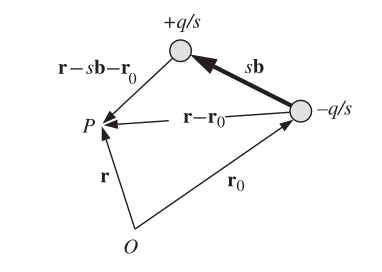
\includegraphics[width=\linewidth]{4p5.png}

\scriptsize

Figura 4.5: Um dipolo com carga total \(Q=0\) e momento de dipolo
\(\mathbf p=q\mathbf b\). O potencial é medido no ponto de observação
\(P\). \(O\) é a origem das coordenadas.

\end{columns}

\end{frame}

%=================================================
\begin{frame}{Densidade de Carga do Dipolo Pontual}

\begin{mybox}{Usando a equação de Poisson}
A densidade de carga associada ao dipolo pontual pode ser obtida a partir de
\[
\rho_D(\mathbf r)=-\epsilon_0\nabla^2\varphi(\mathbf r).
\]
\end{mybox}

\begin{eqbox}
\begin{equation}
\rho_D(\mathbf r)
=
-\mathbf p\cdot\nabla\delta(\mathbf r-\mathbf r_0)
\tag{4.14}
\end{equation}
\end{eqbox}

\begin{alertblock}{Comentário}
Essa densidade é singular: ela não descreve um dipolo físico real, mas é uma
idealização matemática útil.
\end{alertblock}

\notas{pag: 16-20}
\end{frame}

%=================================================
\begin{frame}{4.2.2 A Singularidade na Origem}

\begin{mybox}{Problema}
Para \(\mathbf r\neq \mathbf r_0\), o campo do dipolo pontual é dado pela expressão
usual do campo dipolar.
\end{mybox}

\begin{alertblock}{Questão}
O que acontece exatamente no ponto \(\mathbf r=\mathbf r_0\)?
\end{alertblock}

\begin{mybox}{Ideia}
Como o dipolo pontual foi construído a partir de cargas pontuais, esperamos que
também apareça uma função delta no campo elétrico.
\end{mybox}

\end{frame}

%=================================================
\begin{frame}{Contribuição Singular do Campo}

\begin{mybox}{Resultado da integração esférica}
Para um volume esférico centrado em \(\mathbf r_0\), obtém-se:
\end{mybox}

\begin{eqbox}
\begin{equation}
\int_V d^3r\,\mathbf E(\mathbf r)
=
-\frac{\mathbf p}{3\epsilon_0}
\tag{4.15}
\end{equation}
\end{eqbox}

\begin{alertblock}{Significado}
O campo dipolar regular, sozinho, não captura completamente o comportamento no
ponto singular.
\end{alertblock}

\end{frame}

%=================================================
\begin{frame}{Campo Completo do Dipolo Pontual}

\begin{eqbox}
\begin{equation}
\mathbf E(\mathbf r)
=
\frac{1}{4\pi\epsilon_0}
\left[
\frac{3\hat{\mathbf n}(\hat{\mathbf n}\cdot\mathbf p)-\mathbf p}
{|\mathbf r-\mathbf r_0|^3}
-
\frac{4\pi}{3}\mathbf p\,\delta(\mathbf r-\mathbf r_0)
\right]
\tag{4.16}
\end{equation}
\end{eqbox}

\begin{mybox}{Onde}
\[
\hat{\mathbf n}
=
\frac{\mathbf r-\mathbf r_0}{|\mathbf r-\mathbf r_0|}.
\]
\end{mybox}

\begin{alertblock}{Mensagem}
O termo com delta corrige o campo exatamente na posição do dipolo.
\end{alertblock}

\end{frame}

%=================================================
\begin{frame}{4.2.3 A Força sobre um Dipolo}

\begin{mybox}{Campo externo lentamente variável}
Considere uma distribuição neutra de carga \(\rho(\mathbf r')\) submetida a um campo
externo \(\mathbf E(\mathbf r')\) que varia lentamente no espaço.
\end{mybox}

\begin{eqbox}
\begin{equation}
\mathbf E(\mathbf r')
=
\mathbf E(\mathbf r)
+
[(\mathbf r'-\mathbf r)\cdot\nabla]\mathbf E(\mathbf r)
+\cdots
\tag{4.17}
\end{equation}
\end{eqbox}

\begin{alertblock}{Ideia}
Expandimos o campo em torno de um ponto de referência dentro da distribuição.
\end{alertblock}

\end{frame}

%=================================================
\begin{frame}{Primeira Contribuição Não Nula}

\begin{mybox}{Distribuição neutra}
Como a carga total é zero, o termo constante da expansão não contribui para a
força total.
\end{mybox}

\begin{eqbox}
\begin{equation}
\mathbf F
=
\int d^3r'\,\rho(\mathbf r')\mathbf E(\mathbf r')
=
\int d^3r'\,\rho(\mathbf r')
(\mathbf r'\cdot\nabla)\mathbf E(\mathbf r)
\tag{4.18}
\end{equation}
\end{eqbox}

\begin{alertblock}{Consequência}
A força depende do momento de dipolo da distribuição.
\end{alertblock}
\notas{pag. 25-27}
\end{frame}

%=================================================
\begin{frame}{Força Dipolar}

\begin{eqbox}
\begin{equation}
\mathbf F
=
(\mathbf p\cdot\nabla)\mathbf E(\mathbf r)
\tag{4.19}
\end{equation}
\end{eqbox}

\begin{mybox}{Leitura física}
A força aparece quando o campo elétrico muda de ponto para ponto.
\end{mybox}

\begin{alertblock}{Conclusão importante}
Um campo elétrico uniforme pode produzir torque em um dipolo, mas não produz
força resultante sobre um dipolo neutro.
\end{alertblock}

\end{frame}

%=================================================
\begin{frame}{Forma Alternativa da Força}

\begin{mybox}{Quando \(\mathbf p\) é constante}
Se \(\nabla\times\mathbf E=0\) e \(\mathbf p\) não depende da posição, então:
\end{mybox}

\begin{eqbox}
\begin{equation}
\mathbf F
=
\nabla(\mathbf p\cdot\mathbf E)
\tag{4.20}
\end{equation}
\end{eqbox}

\begin{alertblock}{Interpretação}
A força aponta na direção em que a energia de interação varia mais rapidamente.
\end{alertblock}
\notas{pag. 28-31}
\end{frame}

%=================================================
\begin{frame}{Derivação com a Densidade Singular}

\begin{mybox}{Dipolo pontual equivalente}
A força também pode ser calculada usando a densidade singular do dipolo pontual.
\end{mybox}

\begin{eqbox}
\begin{equation}
\mathbf F
=
\int d^3r'\,\mathbf E(\mathbf r')\rho_D(\mathbf r')
=
\mathbf p\cdot
\int d^3r'\,\delta(\mathbf r'-\mathbf r)\nabla'\mathbf E(\mathbf r')
\tag{4.21}
\end{equation}
\end{eqbox}

\begin{alertblock}{Resultado}
A função delta seleciona o valor local do gradiente do campo.
\end{alertblock}
\notas{pag 31-32}
\end{frame}

\begin{frame}
    \begin{figure}
        \centering
        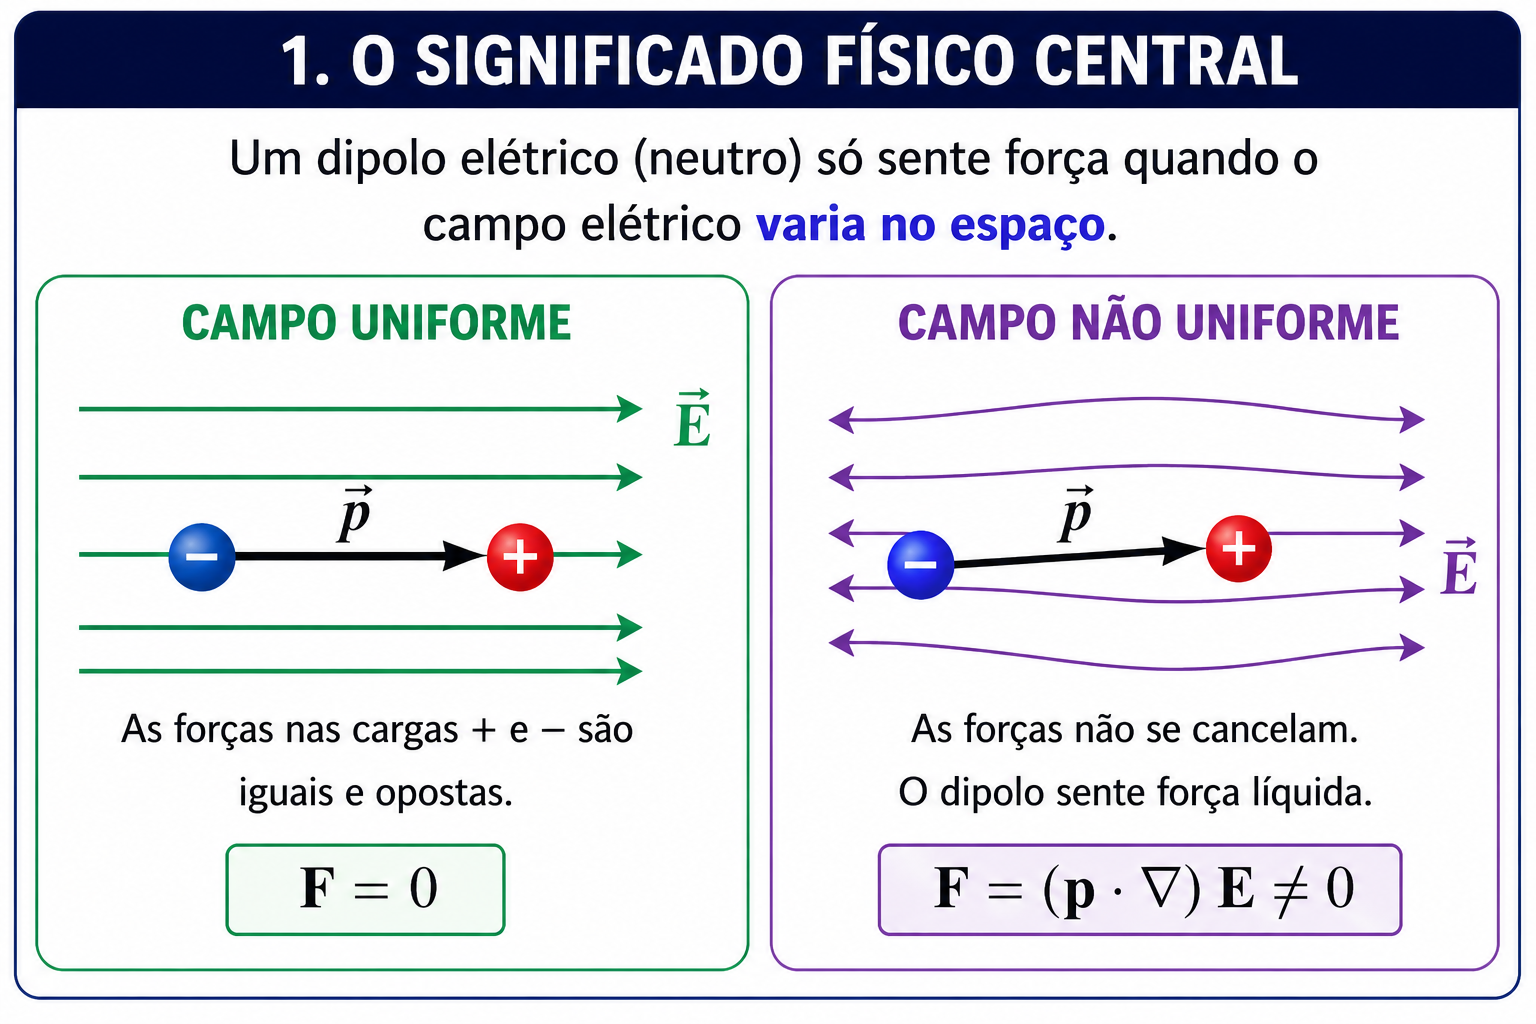
\includegraphics[width=0.8\linewidth]{1.png}

    \end{figure}
\end{frame}

\begin{frame}
    \begin{figure}
        \centering
        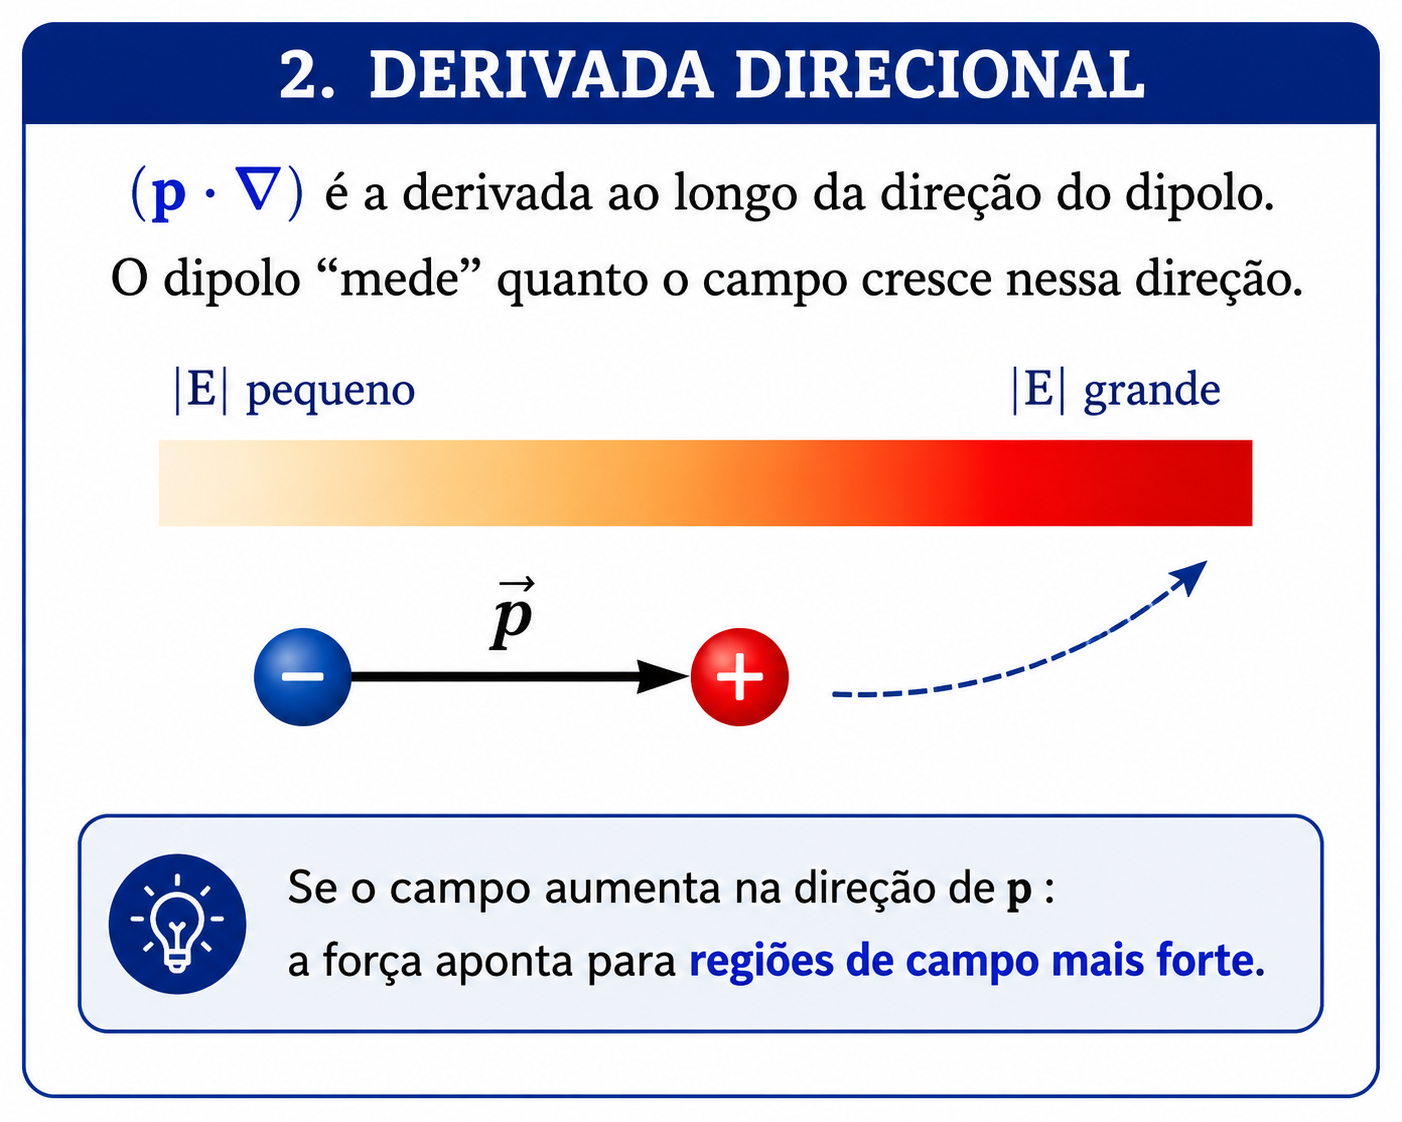
\includegraphics[width=0.7\linewidth]{2.png}

    \end{figure}
\end{frame}

\begin{frame}
    \begin{figure}
        \centering
        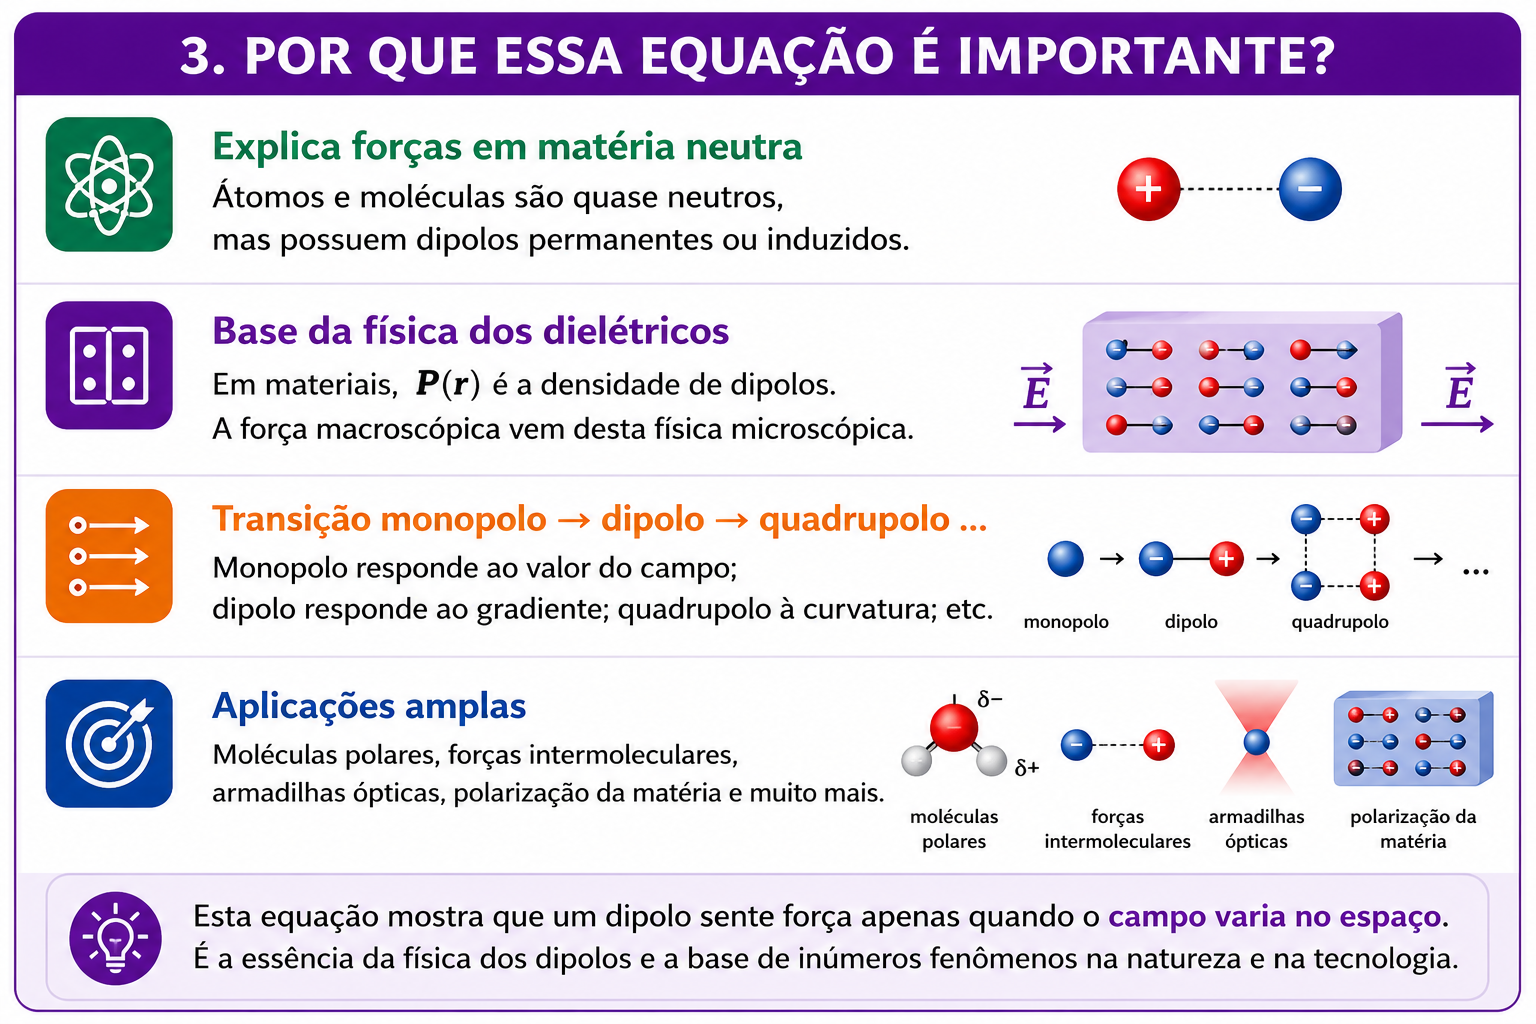
\includegraphics[width=0.8\linewidth]{3.png}

    \end{figure}
\end{frame}

\begin{frame}
    \begin{figure}
        \centering
        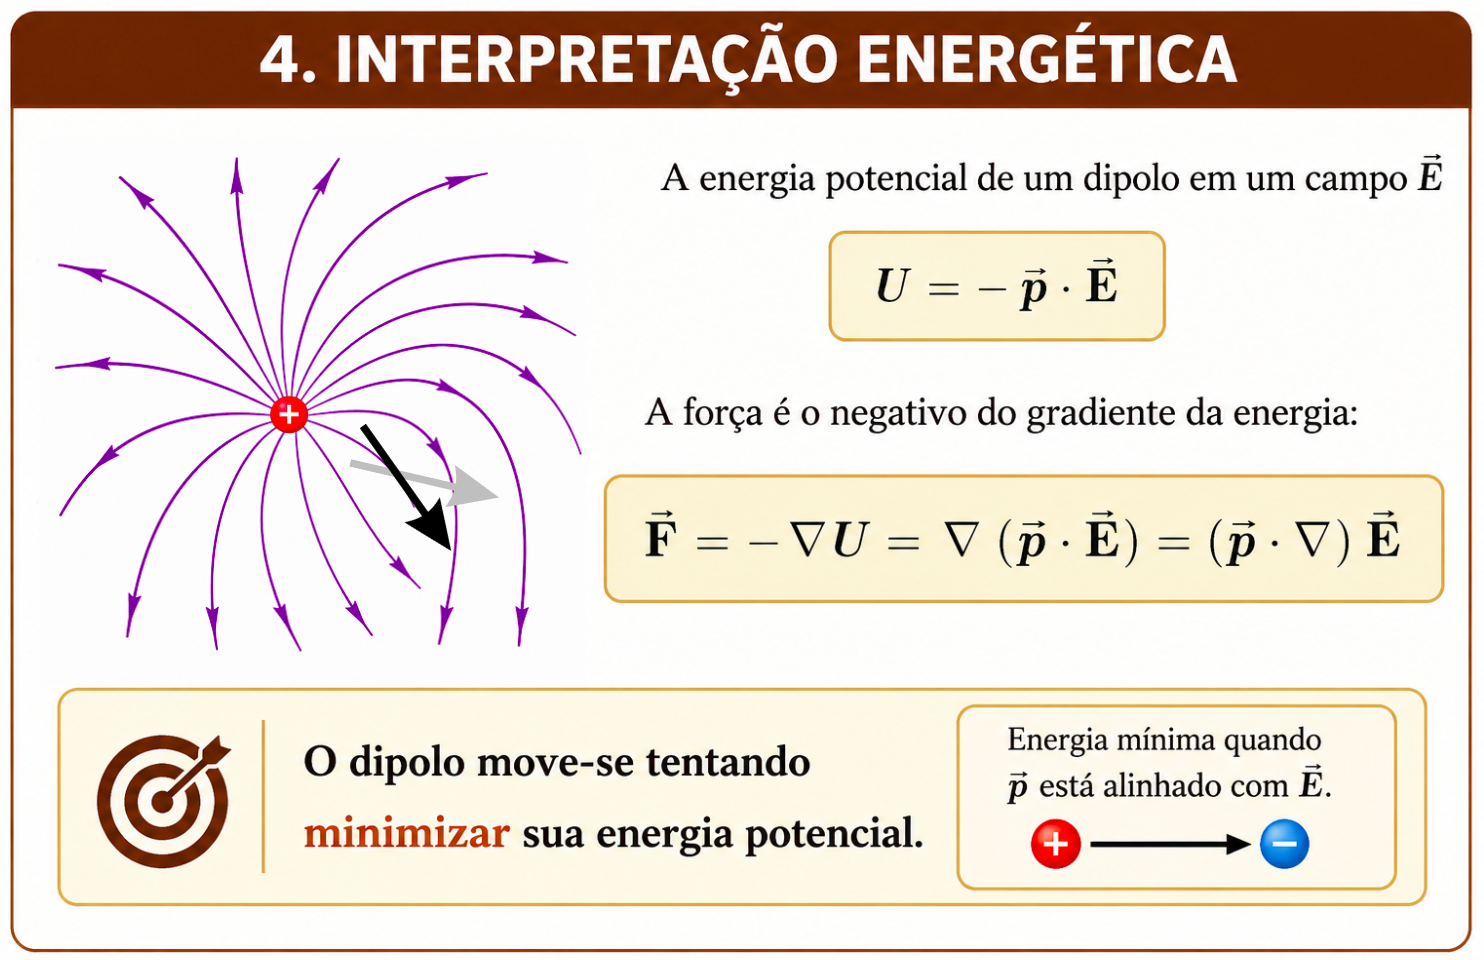
\includegraphics[width=0.8\linewidth]{4.png}

    \end{figure}
\end{frame}

%=================================================
\begin{frame}{4.2.4 O Torque sobre um Dipolo}

\begin{mybox}{Torque de Coulomb}
De modo análogo à força, calculamos o torque exercido pelo campo elétrico sobre
a distribuição dipolar.
\end{mybox}

\begin{eqbox}
\begin{equation}
\mathbf N
=
\int d^3r'\,
\mathbf r'\times\mathbf E(\mathbf r')\rho_D(\mathbf r')
\tag{4.22}
\end{equation}
\end{eqbox}

\begin{alertblock}{Ideia}
O torque mede a tendência do campo em girar a distribuição de carga.
\end{alertblock}
\notas{pag 33-35}
\end{frame}



%=================================================
\begin{frame}{Forma Geral do Torque}

\begin{eqbox}
\begin{equation}
\mathbf N
=
\mathbf p\times\mathbf E
+
\mathbf r\times\mathbf F
\tag{4.24}
\end{equation}
\end{eqbox}

\begin{mybox}{Dois efeitos}
O primeiro termo gira o dipolo em torno de seu próprio centro.

O segundo termo gira o centro da distribuição em torno da origem escolhida.
\end{mybox}

\begin{alertblock}{Caso simples}
Se a origem está no centro do dipolo, o termo \(\mathbf r\times\mathbf F\) desaparece.
\end{alertblock}

\end{frame}

%=================================================
\begin{frame}{Torque em Campo Uniforme}

\begin{mybox}{Campo uniforme}
Quando o campo elétrico é uniforme, a força resultante sobre o dipolo é nula:
\[
\mathbf F=0.
\]
\end{mybox}

\begin{eqbox}
\begin{equation}
\mathbf N
=
\mathbf p\times\mathbf E
\tag{4.24a}
\end{equation}
\end{eqbox}

\begin{alertblock}{Interpretação física}
O campo tende a alinhar o momento de dipolo \(\mathbf p\) com o campo elétrico
\(\mathbf E\).
\end{alertblock}

\end{frame}


%-------------------------------------------------
\begin{frame}{4.2.5 Energia Potencial de um Dipolo}

\begin{mybox}{Ideia física}
A energia de interação entre uma distribuição localizada \(\rho(\mathbf r)\)
e um campo externo lentamente variável pode ser calculada usando a densidade
singular de um dipolo pontual.
\end{mybox}

\begin{eqbox}
\begin{equation}
V_E(\mathbf r)
=
\int d^3r'\,\varphi(\mathbf r')\rho_D(\mathbf r')
=
-\int d^3r'\,\varphi(\mathbf r')\,
\mathbf p\cdot \nabla'\delta(\mathbf r'-\mathbf r).
\tag{4.25}
\label{eq:4.25}
\end{equation}
\end{eqbox}

\begin{mybox}{Observação}
Aqui \(\nabla'\) deriva em relação a \(\mathbf r'\), enquanto \(\mathbf r\) é a posição
do dipolo.
\end{mybox}

\end{frame}

%-------------------------------------------------
\begin{frame}{Integração por Partes}

Partimos de

\begin{equation}
V_E(\mathbf r)
=
-\int d^3r'\,\varphi(\mathbf r')\,
\mathbf p\cdot \nabla'\delta(\mathbf r'-\mathbf r).
\end{equation}

Como \(\mathbf p\) é constante,

\begin{align}
V_E(\mathbf r)
&=
-\sum_i p_i \int d^3r'\,
\varphi(\mathbf r')\,
\partial_i'\delta(\mathbf r'-\mathbf r)
\\[0.2cm]
&=
\sum_i p_i \int d^3r'\,
\delta(\mathbf r'-\mathbf r)\,
\partial_i'\varphi(\mathbf r')
\\[0.2cm]
&=
\mathbf p\cdot \nabla \varphi(\mathbf r).
\end{align}

\end{frame}

%-------------------------------------------------
\begin{frame}{Energia Potencial do Dipolo}

Como

\begin{equation}
\mathbf E(\mathbf r)
=
-\nabla \varphi(\mathbf r),
\end{equation}

temos

\begin{eqbox}
\begin{equation}
V_E(\mathbf r)
=
-\mathbf p\cdot \mathbf E(\mathbf r).
\tag{4.26}
\label{eq:4.26}
\end{equation}
\end{eqbox}

\begin{mybox}{Interpretação}
A energia é mínima quando \(\mathbf p\) está alinhado com \(\mathbf E\).
\end{mybox}

\end{frame}

%-------------------------------------------------
\begin{frame}{Força sobre um Dipolo}

A força é obtida a partir do gradiente negativo da energia:

\begin{align}
\mathbf F
&=
-\nabla V_E
\\[0.2cm]
&=
-\nabla\left[-\mathbf p\cdot \mathbf E(\mathbf r)\right]
\\[0.2cm]
&=
\nabla\left(\mathbf p\cdot \mathbf E\right).
\end{align}

\begin{eqbox}
\begin{equation}
\mathbf F
=
-\nabla V_E
=
\nabla(\mathbf p\cdot \mathbf E).
\tag{4.27}
\label{eq:4.27}
\end{equation}
\end{eqbox}

\begin{mybox}{Comentário}
Se o campo é uniforme, \(\nabla(\mathbf p\cdot \mathbf E)=0\), portanto não há força resultante.
\end{mybox}

\end{frame}

%-------------------------------------------------
\begin{frame}{Rotação Infinitesimal do Dipolo}

Para encontrar o torque, fazemos o dipolo girar rigidamente por um ângulo
infinitesimal \(\delta\boldsymbol{\alpha}\).

\begin{eqbox}
\begin{equation}
\delta \mathbf p
=
\delta\boldsymbol{\alpha}\times \mathbf p.
\tag{4.28}
\label{eq:4.28}
\end{equation}
\end{eqbox}

\begin{mybox}{Ideia}
Uma rotação infinitesimal muda a direção de \(\mathbf p\), mas não muda seu módulo.
\end{mybox}

\end{frame}

%-------------------------------------------------
\begin{frame}{Torque sobre o Dipolo}

A variação da energia é

\begin{align}
\delta V_E
&=
-\delta \mathbf p\cdot \mathbf E
\\[0.2cm]
&=
-(\delta\boldsymbol{\alpha}\times \mathbf p)\cdot \mathbf E
\\[0.2cm]
&=
-(\mathbf p\times \mathbf E)\cdot \delta\boldsymbol{\alpha}.
\end{align}

\begin{eqbox}
\begin{equation}
\delta V_E
=
-\delta \mathbf p\cdot \mathbf E
=
-(\delta\boldsymbol{\alpha}\times \mathbf p)\cdot \mathbf E
=
-(\mathbf p\times \mathbf E)\cdot \delta\boldsymbol{\alpha}.
\tag{4.29}
\label{eq:4.29}
\end{equation}
\end{eqbox}

\end{frame}

%-------------------------------------------------
\begin{frame}{Identificação do Torque}

Pela mecânica,

\begin{equation}
\delta V_E
=
-\mathbf N\cdot \delta\boldsymbol{\alpha}.
\end{equation}

Comparando com

\begin{equation}
\delta V_E
=
-(\mathbf p\times \mathbf E)\cdot \delta\boldsymbol{\alpha},
\end{equation}

obtemos

\begin{eqbox}
\begin{equation}
\mathbf N
=
\mathbf p\times \mathbf E.
\tag{4.24}
\label{eq:4.24}
\end{equation}
\end{eqbox}

\begin{mybox}{Interpretação}
O torque tende a alinhar o dipolo com o campo elétrico.
\end{mybox}

\end{frame}

%-------------------------------------------------
\begin{frame}{4.2.6 Interação Dipolo--Dipolo}

Considere dois dipolos pontuais pré-existentes:

\[
\mathbf p_1 \quad \text{em} \quad \mathbf r_1,
\qquad
\mathbf p_2 \quad \text{em} \quad \mathbf r_2.
\]

\begin{mybox}{Energia de montagem}
Não custa energia trazer o primeiro dipolo para sua posição.

A energia aparece ao trazer o segundo dipolo para o campo produzido pelo primeiro.
\end{mybox}

\begin{equation}
W_{12}
=
-\mathbf p_2\cdot \mathbf E_1(\mathbf r_2).
\end{equation}

\end{frame}

%-------------------------------------------------
\begin{frame}{Campo do Primeiro Dipolo}

Definimos

\begin{equation}
\mathbf R
=
\mathbf r_2-\mathbf r_1,
\qquad
R=
|\mathbf r_2-\mathbf r_1|.
\end{equation}

O campo produzido por \(\mathbf p_1\) no ponto \(\mathbf r_2\) é

\begin{equation}
\mathbf E_1(\mathbf r_2)
=
\frac{1}{4\pi\epsilon_0}
\left[
\frac{3(\mathbf p_1\cdot \mathbf R)\mathbf R}{R^5}
-
\frac{\mathbf p_1}{R^3}
\right].
\end{equation}

Portanto,

\begin{equation}
W_{12}
=
-\mathbf p_2\cdot \mathbf E_1(\mathbf r_2).
\end{equation}

\end{frame}

%-------------------------------------------------
\begin{frame}{Energia de Interação entre Dois Dipolos}

Substituindo o campo de \(\mathbf p_1\), obtemos

\begin{eqbox}
\begin{equation}
W_{12}
=
-\mathbf p_2\cdot \mathbf E_1(\mathbf r_2)
=
\frac{1}{4\pi\epsilon_0}
\left[
\frac{\mathbf p_1\cdot \mathbf p_2}{|\mathbf r_2-\mathbf r_1|^3}
-
\frac{
3\mathbf p_1\cdot(\mathbf r_2-\mathbf r_1)
\mathbf p_2\cdot(\mathbf r_2-\mathbf r_1)
}
{|\mathbf r_2-\mathbf r_1|^5}
\right].
\tag{4.30}
\label{eq:4.30}
\end{equation}
\end{eqbox}

\end{frame}

%-------------------------------------------------
\begin{frame}{Energia Total de Muitos Dipolos}

Para uma coleção de \(N\) dipolos pontuais, somamos a interação de todos os pares:

\begin{eqbox}
\begin{equation}
U_E
=
W
=
\frac{1}{4\pi\epsilon_0}
\frac{1}{2}
\sum_{i=1}^{N}
\sum_{\substack{j=1 \\ j\neq i}}^{N}
\left[
\frac{\mathbf p_i\cdot \mathbf p_j}{|\mathbf r_i-\mathbf r_j|^3}
-
\frac{
3\mathbf p_i\cdot(\mathbf r_i-\mathbf r_j)
\mathbf p_j\cdot(\mathbf r_i-\mathbf r_j)
}
{|\mathbf r_i-\mathbf r_j|^5}
\right].
\tag{4.31}
\label{eq:4.31}
\end{equation}
\end{eqbox}

\end{frame}

%-------------------------------------------------
\begin{frame}{Por que aparece o fator \(1/2\)?}

Na soma dupla,

\[
(i,j)
\qquad \text{e} \qquad
(j,i)
\]

representam o mesmo par físico de dipolos.

\begin{mybox}{Exemplo}
A interação entre os dipolos \(1\) e \(2\) aparece duas vezes:
\[
W_{12}
\quad \text{e} \quad
W_{21}.
\]
\end{mybox}

Por isso dividimos por \(2\):

\begin{equation}
U_E
=
\frac{1}{2}
\sum_{i}
\sum_{j\neq i}
W_{ij}.
\end{equation}

\end{frame}

%-------------------------------------------------
\begin{frame}{Forma Compacta da Energia Total}

Se \(\mathbf E(\mathbf r_i)\) é o campo produzido por todos os outros dipolos
na posição do dipolo \(i\), então

\begin{eqbox}
\begin{equation}
U_E
=
-\frac{1}{2}
\sum_{i=1}^{N}
\mathbf p_i\cdot \mathbf E(\mathbf r_i).
\tag{4.32}
\label{eq:4.32}
\end{equation}
\end{eqbox}

\begin{mybox}{Importante}
O campo \(\mathbf E(\mathbf r_i)\) não inclui o campo do próprio dipolo \(i\).
Ele inclui apenas os campos dos outros dipolos.
\end{mybox}

\end{frame}

%=================================================
\section{Camadas de Dipolos Elétricos}

%-------------------------------------------------
\begin{frame}[plain,noframenumbering]
\begin{tikzpicture}[remember picture,overlay]
    \fill[myblue] (current page.south west) rectangle (current page.north east);
    \fill[mycyan!35] ([xshift=-1.2cm,yshift=-1.0cm]current page.north east) circle (3.2cm);
    \fill[mycyan!20] ([xshift=1.0cm,yshift=0.8cm]current page.south west) circle (3.8cm);
\end{tikzpicture}

\vspace{1.8cm}

\begin{center}
{\color{white}\Huge \textbf{4.3 Camadas de Dipolos Elétricos}}

\vspace{0.5cm}

{\color{white}\Large Densidade superficial de momento de dipolo}

\vspace{1.0cm}

{\color{white}\large Potencial, densidade singular de carga e salto no potencial}
\end{center}

\end{frame}

%-------------------------------------------------
\begin{frame}{Ideia Física: Camada de Dipolos}

\begin{mybox}{Definição informal}
Uma camada de dipolos é uma distribuição de dipolos elétricos confinados a uma superfície.
\end{mybox}

\begin{itemize}
\item Cada molécula possui momento de dipolo \(\mathbf p\).
\item Muitas moléculas próximas formam uma distribuição superficial.
\item A grandeza macroscópica relevante é o momento de dipolo por unidade de área.
\end{itemize}

\begin{eqbox}
\begin{equation}
\boldsymbol{\tau}
=
\frac{\mathbf p}{S}
=
\frac{q\mathbf b}{S}
=
\sigma \mathbf b .
\tag{4.33}
\label{eq:4.33}
\end{equation}
\end{eqbox}

\end{frame}

%-------------------------------------------------
\begin{frame}{Representação por Duas Superfícies Carregadas}

\begin{center}
\begin{tikzpicture}[scale=1.15]

% placas
\draw[thick] (-3,0.45) -- (3,0.45);
\draw[thick] (-3,-0.45) -- (3,-0.45);

% labels charges
\node at (0,0.75) {\Large \(+\sigma\)};
\node at (0,-0.75) {\Large \(-\sigma\)};

% separation b
\draw[<->,thick] (-3.35,-0.45) -- (-3.35,0.45);
\node[left] at (-3.35,0) {\Large \(b\)};

% dipole density arrow
\draw[->,very thick,myblue] (3.35,-0.45) -- (3.35,0.45);
\node[right] at (3.45,0) {\Large \(\boldsymbol{\tau}=\sigma\mathbf b\)};

\end{tikzpicture}
\end{center}

\begin{mybox}{Figura 4.7}
Vista lateral de uma camada de dipolos: duas superfícies com densidades de carga opostas \(\pm\sigma\), separadas por uma distância \(b\).
\end{mybox}

\end{frame}

%-------------------------------------------------
\begin{frame}{Limite Macroscópico da Camada}

\begin{mybox}{Limite de camada fina}
Tomamos
\[
b\to 0,
\qquad
\sigma\to \infty,
\qquad
\boldsymbol{\tau}=\sigma\mathbf b
\quad \text{fixo}.
\]
\end{mybox}

\begin{itemize}
\item A separação microscópica entre as cargas deixa de ser resolvida.
\item A camada passa a ser descrita apenas por \(\boldsymbol{\tau}\).
\item \(\boldsymbol{\tau}\) é uma propriedade superficial, assim como \(\sigma\).
\end{itemize}

\end{frame}

%-------------------------------------------------
\begin{frame}{4.3.1 Potencial de uma Camada de Dipolos}

Para uma superfície \(S\), generalizamos a densidade de momento de dipolo:

\begin{eqbox}
\begin{equation}
\boldsymbol{\tau}
=
\frac{d\mathbf p}{dS}.
\tag{4.34}
\label{eq:4.34}
\end{equation}
\end{eqbox}

\begin{mybox}{Caso geral}
A superfície não precisa ser plana, \(\boldsymbol{\tau}\) não precisa ser uniforme e os dipolos não precisam ser perpendiculares à superfície.
\end{mybox}

\end{frame}

%-------------------------------------------------
\begin{frame}{Potencial por Superposição de Dipolos Pontuais}

O potencial de uma camada é obtido somando os potenciais de dipolos pontuais:

\begin{eqbox}
\begin{equation}
\varphi(\mathbf r)
=
-\frac{1}{4\pi\epsilon_0}
\int_S
d\mathbf p(\mathbf r_s)\cdot
\nabla
\frac{1}{|\mathbf r-\mathbf r_s|}.
\tag{4.35a}
\label{eq:4.35a}
\end{equation}
\end{eqbox}

Como

\[
d\mathbf p(\mathbf r_s)=\boldsymbol{\tau}(\mathbf r_s)dS,
\]

temos

\begin{eqbox}
\begin{equation}
\varphi(\mathbf r)
=
-\frac{1}{4\pi\epsilon_0}
\int_S
dS\,
\boldsymbol{\tau}(\mathbf r_s)\cdot
\nabla
\frac{1}{|\mathbf r-\mathbf r_s|}.
\tag{4.35}
\label{eq:4.35}
\end{equation}
\end{eqbox}

\end{frame}

%-------------------------------------------------
\begin{frame}{Convertendo a Integral de Superfície em Volume}

Para uma camada no plano \(z=0\), escrevemos

\[
\mathbf r'_s=x'\hat{\mathbf x}+y'\hat{\mathbf y},
\qquad
\mathbf r'
=
\mathbf r'_s+z'\hat{\mathbf z}.
\]

A superfície pode ser representada por uma delta de Dirac:

\begin{eqbox}
\begin{equation}
\varphi(\mathbf r)
=
-\frac{1}{4\pi\epsilon_0}
\int
d^3r'\,
\delta(z')\,
\boldsymbol{\tau}(\mathbf r'_s)\cdot
\nabla
\frac{1}{|\mathbf r-\mathbf r'|}.
\tag{4.36}
\label{eq:4.36}
\end{equation}
\end{eqbox}

\end{frame}

%-------------------------------------------------
\begin{frame}{Mudando o Gradiente de \(\mathbf r\) para \(\mathbf r'\)}

Usamos a identidade

\begin{equation}
\nabla
\frac{1}{|\mathbf r-\mathbf r'|}
=
-\nabla'
\frac{1}{|\mathbf r-\mathbf r'|}.
\end{equation}

Assim,

\begin{align}
\varphi(\mathbf r)
&=
-\frac{1}{4\pi\epsilon_0}
\int d^3r'\,
\delta(z')\boldsymbol{\tau}(\mathbf r'_s)\cdot
\nabla
\frac{1}{|\mathbf r-\mathbf r'|}
\\
&=
\frac{1}{4\pi\epsilon_0}
\int d^3r'\,
\delta(z')\boldsymbol{\tau}(\mathbf r'_s)\cdot
\nabla'
\frac{1}{|\mathbf r-\mathbf r'|}.
\end{align}

\end{frame}

%-------------------------------------------------
\begin{frame}{Integração por Partes}

Definindo

\[
\mathbf A(\mathbf r')
=
\boldsymbol{\tau}(\mathbf r'_s)\delta(z'),
\]

temos

\begin{equation}
\int d^3r'\,
\mathbf A\cdot\nabla'
\frac{1}{|\mathbf r-\mathbf r'|}
=
-
\int d^3r'\,
\frac{\nabla'\cdot\mathbf A}{|\mathbf r-\mathbf r'|}.
\end{equation}

Logo,

\begin{eqbox}
\begin{equation}
\varphi(\mathbf r)
=
-\frac{1}{4\pi\epsilon_0}
\int
d^3r'\,
\frac{
\nabla'\cdot
\left[
\boldsymbol{\tau}(\mathbf r'_s)\delta(z')
\right]
}
{|\mathbf r-\mathbf r'|}.
\tag{4.37}
\label{eq:4.37}
\end{equation}
\end{eqbox}

\end{frame}

%-------------------------------------------------
\begin{frame}{Densidade Singular de Carga da Camada}

Comparando com

\begin{equation}
\varphi(\mathbf r)
=
\frac{1}{4\pi\epsilon_0}
\int d^3r'\,
\frac{\rho(\mathbf r')}{|\mathbf r-\mathbf r'|},
\end{equation}

identificamos

\begin{eqbox}
\begin{equation}
\rho_L(\mathbf r)
=
-\nabla\cdot
\left[
\boldsymbol{\tau}(\mathbf r_s)\delta(z)
\right].
\tag{4.38}
\label{eq:4.38}
\end{equation}
\end{eqbox}

\begin{mybox}{Interpretação}
Uma camada de dipolos é equivalente a uma distribuição singular de carga localizada na superfície.
\end{mybox}

\end{frame}

%-------------------------------------------------
\begin{frame}{Figura 4.8: Potencial e Densidade Singular}

\begin{center}
\begin{tikzpicture}
\begin{axis}[
    width=10.5cm,
    height=5.5cm,
    axis lines=middle,
    xmin=-4,
    xmax=4,
    ymin=-1.4,
    ymax=1.4,
    xlabel={\(z\)},
    ylabel={},
    xtick=\empty,
    ytick=\empty,
    clip=false,
    samples=300,
    domain=-4:4,
]

% rho_L(z) ~ derivative of Gaussian
\addplot[very thick,myblue]
{3*x*exp(-4*x^2)};
\node[myblue] at (axis cs:-1.25,-0.40) {\(\rho_L(z)\)};

% potential step
\addplot[very thick,dashed,myred]
{0.75*tanh(1.8*x)};
\node[myred] at (axis cs:1.85,0.92) {\(\varphi(z)\)};

% Delta phi arrow
\draw[<->,thick] (axis cs:4.4,-0.75) -- (axis cs:4.4,0.75);
\node[right] at (axis cs:4.5,0) {\(\Delta\varphi\)};

% vertical layer
\draw[gray,thick] (axis cs:0,-1.2) -- (axis cs:0,1.2);

\end{axis}
\end{tikzpicture}
\end{center}

\begin{mybox}{Mensagem da figura}
No limite macroscópico, \(\rho_L\) torna-se singular em \(z=0\), enquanto o potencial sofre um salto finito \(\Delta\varphi\).
\end{mybox}

\end{frame}

%-------------------------------------------------
\begin{frame}{Gradiente Superficial}

Para interpretar \(\rho_L\), definimos o gradiente superficial:

\begin{eqbox}
\begin{equation}
\nabla_S
=
\hat{\mathbf x}\frac{\partial}{\partial x}
+
\hat{\mathbf y}\frac{\partial}{\partial y}.
\tag{4.39}
\label{eq:4.39}
\end{equation}
\end{eqbox}

\begin{mybox}{Ideia}
\(\nabla_S\) mede variações apenas ao longo da superfície, não na direção perpendicular.
\end{mybox}

\end{frame}

%-------------------------------------------------
\begin{frame}{Carga Superficial Efetiva}

A variação lateral da densidade de dipolos gera uma carga superficial efetiva:

\begin{eqbox}
\begin{equation}
\sigma(\mathbf r_s)
=
-\nabla_S\cdot\boldsymbol{\tau}(\mathbf r_s).
\tag{4.40}
\label{eq:4.40}
\end{equation}
\end{eqbox}

\begin{mybox}{Interpretação}
Se \(\boldsymbol{\tau}\) varia ao longo da superfície, os extremos positivos e negativos dos dipolos paralelos não se cancelam completamente.
\end{mybox}

\end{frame}

%-------------------------------------------------
\begin{frame}{Separando as Contribuições de \(\rho_L\)}

Escrevemos

\[
\boldsymbol{\tau}
=
\boldsymbol{\tau}_\parallel+\tau_z\hat{\mathbf z}.
\]

Então,

\begin{align}
\rho_L(\mathbf r)
&=
-\nabla\cdot
\left[
\boldsymbol{\tau}(\mathbf r_s)\delta(z)
\right]
\\
&=
-\nabla_S\cdot
\left[
\boldsymbol{\tau}_\parallel(\mathbf r_s)\delta(z)
\right]
-
\frac{\partial}{\partial z}
\left[
\tau_z(\mathbf r_s)\delta(z)
\right].
\end{align}

Como \(\boldsymbol{\tau}\) não depende de \(z\),

\begin{eqbox}
\begin{equation}
\rho_L(\mathbf r)
=
-\tau_z(\mathbf r_s)\delta'(z)
+
\sigma(\mathbf r_s)\delta(z).
\tag{4.41}
\label{eq:4.41}
\end{equation}
\end{eqbox}

\end{frame}

%-------------------------------------------------
\begin{frame}{Significado dos Dois Termos}

\begin{eqbox}
\begin{equation}
\rho_L(\mathbf r)
=
-\tau_z(\mathbf r_s)\delta'(z)
+
\sigma(\mathbf r_s)\delta(z).
\tag{4.41}
\end{equation}
\end{eqbox}

\begin{mybox}{Termo perpendicular}
\[
-\tau_z(\mathbf r_s)\delta'(z)
\]
vem da componente do dipolo perpendicular à superfície.
\end{mybox}

\begin{mybox}{Termo paralelo}
\[
\sigma(\mathbf r_s)\delta(z)
\]
vem da variação lateral dos dipolos paralelos à superfície.
\end{mybox}

\end{frame}

%-------------------------------------------------
\begin{frame}{Relação com a Equação de Poisson}

No caso unidimensional,

\begin{eqbox}
\begin{equation}
\epsilon_0
\frac{d^2\varphi(z)}{dz^2}
=
-\rho_L(z).
\tag{4.42}
\label{eq:4.42}
\end{equation}
\end{eqbox}

\begin{mybox}{Leitura física}
A curvatura do potencial está diretamente ligada à densidade de carga.
\end{mybox}

\begin{itemize}
\item Onde \(\rho_L(z)\) é positiva, a curvatura de \(\varphi(z)\) é negativa.
\item Onde \(\rho_L(z)\) é negativa, a curvatura de \(\varphi(z)\) é positiva.
\item No limite de camada infinitamente fina, o potencial apresenta uma descontinuidade.
\end{itemize}

\end{frame}


%-------------------------------------------------
\begin{frame}{4.3.2 Condições de Contorno em uma Camada de Dipolos}

\begin{mybox}{Condição já conhecida}
O termo proporcional a \(\sigma(\mathbf r_s)\delta(z)\) gera uma descontinuidade na componente normal do campo elétrico:
\[
\epsilon_0\hat{\mathbf n}_2\cdot
\left[\mathbf E_1-\mathbf E_2\right]
=
\sigma(\mathbf r_s).
\]
\end{mybox}

Agora queremos entender o efeito do primeiro termo de

\begin{equation}
\rho_L(\mathbf r)
=
-\tau_z(\mathbf r_s)\delta'(z)
+
\sigma(\mathbf r_s)\delta(z).
\tag{4.41}
\end{equation}

\end{frame}

%-------------------------------------------------
\begin{frame}{Equação de Poisson para o Termo \(\delta'(z)\)}

Usando apenas o termo

\[
\rho_L(\mathbf r)
=
-\tau_z(\mathbf r_s)\delta'(z),
\]

a equação de Poisson

\[
\epsilon_0\nabla^2\varphi=-\rho_L
\]

fica, na direção normal à camada,

\begin{eqbox}
\begin{equation}
\epsilon_0
\frac{d^2}{dz^2}
\varphi(\mathbf r_s,z)
=
\tau_z(\mathbf r_s)\delta'(z).
\tag{4.43}
\label{eq:4.43}
\end{equation}
\end{eqbox}

\begin{mybox}{Ideia}
A derivada da delta de Dirac gera uma descontinuidade no próprio potencial.
\end{mybox}

\end{frame}

%-------------------------------------------------
\begin{frame}{Primeira Integração}

Integramos a equação

\[
\epsilon_0
\frac{d^2\varphi}{dz^2}
=
\tau_z(\mathbf r_s)\delta'(z)
\]

uma vez em relação a \(z\):

\begin{eqbox}
\begin{equation}
\epsilon_0
\frac{d}{dz}
\varphi(\mathbf r_s,z)
=
\tau_z(\mathbf r_s)\delta(z)
+
C.
\tag{4.44}
\label{eq:4.44}
\end{equation}
\end{eqbox}

\begin{mybox}{Comentário}
A constante \(C\) desaparece quando calculamos a diferença entre os dois lados imediatamente vizinhos da camada.
\end{mybox}

\end{frame}

%-------------------------------------------------
\begin{frame}{Salto no Potencial}

Integramos (4.44) de \(z=0^-\) até \(z=0^+\):

\begin{align}
\int_{0^-}^{0^+}
\epsilon_0
\frac{d\varphi}{dz}\,dz
&=
\int_{0^-}^{0^+}
\tau_z(\mathbf r_s)\delta(z)\,dz
\\[0.2cm]
\epsilon_0
\left[
\varphi(\mathbf r_s,0^+)
-
\varphi(\mathbf r_s,0^-)
\right]
&=
\tau_z(\mathbf r_s).
\end{align}

\begin{eqbox}
\begin{equation}
\varphi(\mathbf r_s,z=0^+)
-
\varphi(\mathbf r_s,z=0^-)
=
\frac{\tau_z(\mathbf r_s)}{\epsilon_0}.
\tag{4.45}
\label{eq:4.45}
\end{equation}
\end{eqbox}

\end{frame}

%-------------------------------------------------
\begin{frame}{Interpretação do Salto em \(\varphi\)}

\begin{mybox}{Resultado principal}
Uma camada de dipolos produz uma descontinuidade finita no potencial eletrostático.
\end{mybox}

\[
\Delta\varphi
=
\varphi(0^+)-\varphi(0^-)
=
\frac{\tau_z}{\epsilon_0}.
\]

\begin{mybox}{Por quê?}
Dentro da camada microscópica, o campo elétrico aponta da carga positiva para a carga negativa.

Assim, ao atravessar a camada, o potencial muda rapidamente.
\end{mybox}

\end{frame}

%-------------------------------------------------
\begin{frame}{Descontinuidade no Campo Tangencial}

Se a densidade de dipolo varia ao longo da superfície, o campo tangencial também pode ser descontínuo.

\begin{eqbox}
\begin{equation}
\hat{\mathbf n}_2
\times
\left[
\mathbf E_1-\mathbf E_2
\right]
=
\nabla
\times
\left[
\hat{\mathbf n}_2
\left(
\hat{\mathbf n}_2\cdot\boldsymbol{\tau}
\right)
\right]
/
\epsilon_0 .
\tag{4.46}
\label{eq:4.46}
\end{equation}
\end{eqbox}

\begin{mybox}{Comentário físico}
Essa condição altera as fórmulas usuais de reflexão e transmissão quando há uma camada de dipolos na interface.
\end{mybox}

\end{frame}

%=================================================
\section{Aplicação 4.1: Gotas Monocamadas de Dipolos}

%-------------------------------------------------
\begin{frame}[plain,noframenumbering]
\begin{tikzpicture}[remember picture,overlay]
    \fill[myblue] (current page.south west) rectangle (current page.north east);
    \fill[mycyan!35] ([xshift=-1.2cm,yshift=-1.0cm]current page.north east) circle (3.2cm);
    \fill[mycyan!20] ([xshift=1.0cm,yshift=0.8cm]current page.south west) circle (3.8cm);
\end{tikzpicture}

\vspace{1.8cm}

\begin{center}
{\color{white}\Huge \textbf{Aplicação 4.1}}

\vspace{0.5cm}

{\color{white}\Large Gotas Monocamadas de Dipolos Elétricos}

\vspace{1.0cm}

{\color{white}\large Por que todas as gotas têm quase a mesma largura?}
\end{center}

\end{frame}

%-------------------------------------------------
\begin{frame}{Modelo da Gota Retangular}

\begin{mybox}{Hipóteses}
Consideramos uma gota retangular de área fixa
\[
A=Lw,
\]
com comprimento \(L\) e largura \(w\), no regime
\[
L\gg w\gg a.
\]
\end{mybox}

\begin{itemize}
\item \(a\): distância lateral entre moléculas vizinhas;
\item cada molécula possui dipolo apontando para fora da página;
\item queremos encontrar a largura de equilíbrio \(w_0\).
\end{itemize}

\end{frame}

%-------------------------------------------------
\begin{frame}{Figura 4.9: Vista Superior da Gota}

\begin{center}
\begin{tikzpicture}[scale=0.72]

% grade
\draw[step=0.35,gray!60,thin] (0,0) grid (9.8,2.45);

% contorno
\draw[thick] (0,0) rectangle (9.8,2.45);

% linha de moléculas destacada
\foreach \x in {0.175,0.525,...,9.625}
{
    \fill[black] (\x,0.35) circle (0.065);
}

% molécula a distância y
\fill[black] (3.85,1.75) circle (0.075);

% a
\draw[<->,thick] (0.4,2.75) -- (0.0,2.75);
\node[above] at (0.2,2.75) {\(a\)};

% y
\draw[<->,thick] (-0.35,0.35) -- (-0.35,1.75);
\node[left] at (-0.35,1.05) {\(y\)};

% w
\draw[<->,thick] (10.15,0) -- (10.15,2.45);
\node[right] at (10.15,1.225) {\(w\)};

% L
\draw[<->,thick] (0,-0.45) -- (9.8,-0.45);
\node[below] at (4.9,-0.45) {\(L\)};

\end{tikzpicture}
\end{center}

\begin{mybox}{Representação}
Cada quadrado contém uma molécula polar. Os pontos pretos destacam uma linha completa de moléculas e uma molécula a uma distância \(y\) dessa linha.
\end{mybox}

\end{frame}

%-------------------------------------------------
\begin{frame}{Energia de Perímetro}

A energia química é proporcional ao perímetro da gota.

Como \(L\gg w\), o perímetro é aproximadamente

\[
2L.
\]

Se \(\lambda\) é a energia química por unidade de comprimento,

\begin{eqbox}
\begin{equation}
U_C
\approx
2L\lambda
=
\frac{2\lambda A}{w}.
\tag{4.47}
\label{eq:4.47}
\end{equation}
\end{eqbox}

\begin{mybox}{Interpretação}
Para área fixa \(A\), aumentar \(w\) diminui \(L=A/w\), reduzindo a energia de perímetro.
\end{mybox}

\end{frame}

%-------------------------------------------------
\begin{frame}{Energia Eletrostática entre Duas Linhas}

Cada linha contém dipolos paralelos distribuídos ao longo do comprimento \(L\).

A interação entre duas linhas separadas por distância \(y\) é

\begin{eqbox}
\begin{equation}
U(y)
=
\frac{1}{4\pi\epsilon_0}
\int_0^L dx_1
\int_0^L dx_2
\frac{\tau^2a^2}
{\left[(x_1-x_2)^2+y^2\right]^{3/2}}.
\tag{4.48a}
\label{eq:4.48a}
\end{equation}
\end{eqbox}

\begin{mybox}{Origem}
Este termo vem da interação dipolo--dipolo para dipolos perpendiculares ao plano da gota.
\end{mybox}

\end{frame}

%-------------------------------------------------
\begin{frame}{Resultado da Integral entre Linhas}

A integral resulta em

\begin{eqbox}
\begin{equation}
U(y)
=
\frac{\tau^2a^2}{4\pi\epsilon_0}
\frac{2}{y^2}
\left[
\sqrt{L^2+y^2}-y
\right].
\tag{4.48}
\label{eq:4.48}
\end{equation}
\end{eqbox}

No limite

\[
L\gg y,
\]

\end{frame}

\begin{frame}

temos

\begin{equation}
\sqrt{L^2+y^2}\approx L,
\end{equation}

portanto

\begin{eqbox}
\begin{equation}
U(y)
\approx
\frac{\tau^2a^2L}{2\pi\epsilon_0y^2}.
\end{equation}
\end{eqbox}

\end{frame}

%-------------------------------------------------
\begin{frame}{Somando Pares de Linhas}

Há aproximadamente

\[
\frac{w}{a}
\]

linhas paralelas de dipolos.

\begin{mybox}{Contagem dos pares}
\begin{itemize}
\item \(w/a-1\) pares separados por \(a\);
\item \(w/a-2\) pares separados por \(2a\);
\item \(w/a-n\) pares separados por \(na\).
\end{itemize}
\end{mybox}

Assim,

\[
y=na.
\]

\end{frame}

%-------------------------------------------------
\begin{frame}{Energia Eletrostática Total}

Somando todos os pares de linhas,

\begin{eqbox}
\begin{equation}
U_E
=
\frac{\tau^2L}{2\pi\epsilon_0}
\sum_{n=1}^{w/a}
\frac{w/a-n}{n^2}.
\tag{4.49a}
\label{eq:4.49a}
\end{equation}
\end{eqbox}

Para \(w\gg a\), aproximamos a soma por uma integral:

\begin{eqbox}
\begin{equation}
U_E
\approx
\frac{\tau^2L}{2\pi\epsilon_0}
\int_1^{w/a}
dn\,
\frac{w/a-n}{n^2}.
\tag{4.49b}
\label{eq:4.49b}
\end{equation}
\end{eqbox}

\end{frame}

%-------------------------------------------------
\begin{frame}{Cálculo da Integral}

Calculamos

\begin{align}
\int_1^{w/a}
\frac{w/a-n}{n^2}\,dn
&=
\frac{w}{a}
\int_1^{w/a}
\frac{dn}{n^2}
-
\int_1^{w/a}
\frac{dn}{n}
\\[0.2cm]
&=
\frac{w}{a}
\left[
1-\frac{a}{w}
\right]
-
\ln\frac{w}{a}
\\[0.2cm]
&\approx
\frac{w}{a}
-
\ln\frac{w}{a}.
\end{align}

Logo,

\begin{eqbox}
\begin{equation}
U_E
\approx
\frac{\tau^2L}{2\pi\epsilon_0}
\left[
\frac{w}{a}
-
\ln\frac{w}{a}
\right].
\tag{4.49}
\label{eq:4.49}
\end{equation}
\end{eqbox}

\end{frame}

%-------------------------------------------------
\begin{frame}{Energia Total da Gota}

A energia total é a soma de

\[
U_T=U_C+U_E.
\]

Usando

\[
L=\frac{A}{w},
\]

temos

\begin{eqbox}
\begin{equation}
U_T
=
U_C+U_E
=
\frac{2A}{w}
\left[
\lambda
+
\frac{\tau^2}{4\pi\epsilon_0}
\left(
\frac{w}{a}
-
\ln\frac{w}{a}
\right)
\right].
\tag{4.50}
\label{eq:4.50}
\end{equation}
\end{eqbox}

\end{frame}

%-------------------------------------------------
\begin{frame}{Minimização da Energia}

Queremos minimizar

\[
U_T(w)
=
\frac{2A}{w}
\left[
\lambda
+
\frac{\tau^2}{4\pi\epsilon_0}
\left(
\frac{w}{a}
-
\ln\frac{w}{a}
\right)
\right].
\]

Definindo

\[
C=\frac{\tau^2}{4\pi\epsilon_0},
\]

temos

\[
U_T(w)
=
2A
\left[
\frac{\lambda}{w}
+
\frac{C}{a}
-
\frac{C}{w}\ln\frac{w}{a}
\right].
\]

\end{frame}

%-------------------------------------------------
\begin{frame}{Encontrando a Largura de Equilíbrio}

Derivamos em relação a \(w\):

\begin{align}
\frac{dU_T}{dw}
&=
2A
\left[
-\frac{\lambda}{w^2}
-
C\frac{d}{dw}
\left(
\frac{1}{w}\ln\frac{w}{a}
\right)
\right]
\\[0.2cm]
&=
2A
\left[
-\frac{\lambda}{w^2}
-
C
\left(
\frac{1}{w^2}
-
\frac{1}{w^2}\ln\frac{w}{a}
\right)
\right].
\end{align}

No equilíbrio,

\[
\frac{dU_T}{dw}=0.
\]

\end{frame}

%-------------------------------------------------
\begin{frame}{Resultado para \(w_0\)}

Da condição

\[
-\lambda
-
C
+
C\ln\frac{w_0}{a}
=
0,
\]

obtemos

\[
\ln\frac{w_0}{a}
=
1+\frac{\lambda}{C}.
\]

Como

\[
C=\frac{\tau^2}{4\pi\epsilon_0},
\]

segue que

\[
w_0
=
a\exp\left(
1+\frac{4\pi\epsilon_0\lambda}{\tau^2}
\right).
\]
\end{frame}

\begin{frame}

Negligenciando o fator \(e\) na aproximação logarítmica,

\begin{eqbox}
\begin{equation}
w_0
\approx
a\exp\left(
\frac{4\pi\epsilon_0\lambda}{\tau^2}
\right).
\tag{4.51}
\label{eq:4.51}
\end{equation}
\end{eqbox}

\end{frame}

%-------------------------------------------------
\begin{frame}{Interpretação Física do Resultado}

\begin{eqbox}
\begin{equation}
w_0
\approx
a\exp\left(
\frac{4\pi\epsilon_0\lambda}{\tau^2}
\right).
\tag{4.51}
\end{equation}
\end{eqbox}

\begin{mybox}{Consequência importante}
A largura de equilíbrio \(w_0\) é independente do comprimento \(L\) da gota.
\end{mybox}

\begin{itemize}
\item A gota cresce aumentando seu comprimento \(L\).
\item A largura permanece aproximadamente fixa.
\item Isso explica por que as gotas observadas têm praticamente a mesma largura.
\end{itemize}

\end{frame}


%================================================
\section{O Quadrupolo Elétrico}
%================================================
%================================================
\begin{frame}[plain]

\begin{tikzpicture}[remember picture,overlay]

% Fundo
\fill[myblue] (current page.south west)
rectangle
(current page.north east);

% Círculos decorativos
\fill[mycyan!25]
(current page.north east)
circle (3.8cm);

\fill[white!10]
(current page.south west)
circle (2.8cm);

% Linhas multipolares estilizadas
\draw[white, line width=1.5pt]
(-6,-1)
.. controls (-3,1) and (-1,0) ..
(2,2);

\draw[white, line width=1.2pt]
(-6,-2)
.. controls (-2,-1) and (0,1) ..
(4,3);

\draw[white!70, line width=1pt]
(-5,-3)
.. controls (-1,-2) and (1,0) ..
(5,2);

% Pequenos pontos
\fill[myred] (-2,0.3) circle (0.12);
\fill[white] (-1.3,-0.2) circle (0.10);
\fill[myred] (-0.6,0.4) circle (0.12);
\fill[white] (0.2,-0.1) circle (0.10);

% Título
\node[
text width=12cm,
align=center,
text=white
]
at (current page.center)
{
{\Huge\bfseries O Quadrupolo Elétrico}

\vspace{0.4cm}

{\Large Expansão Multipolar e Tensores}

\vspace{0.6cm}

{\large Física Matemática do Momento de Quadrupolo}
};

% Fórmula decorativa
\node[
text=white,
scale=1.5
]
at ($(current page.center)+(0,-3.0)$)
{
$
\varphi(\mathbf r)
=
\frac{1}{4\pi\epsilon_0}
Q_{ij}
\frac{3r_i r_j-\delta_{ij}r^2}{r^5}
$
};

\end{tikzpicture}

\end{frame}
%================================================
%------------------------------------------------
\begin{frame}{Quando o Quadrupolo Domina}

\begin{mybox}{Ideia Física}
O termo de quadrupolo domina quando:
\[
Q=0
\qquad\text{e}\qquad
\mathbf p =0.
\]
Ou seja:
\begin{itemize}
\item carga total nula;
\item momento de dipolo nulo.
\end{itemize}
\end{mybox}
\end{frame}

\begin{frame}


\begin{alertblock}{Exemplos}
\begin{itemize}
\item núcleos atômicos;
\item moléculas diatômicas homonucleares (\(\mathrm{N}_2\), por exemplo).
\end{itemize}
\end{alertblock}

\begin{eqbox}
\begin{equation}
\varphi(\mathbf r)
=
\frac{1}{4\pi\epsilon_0}
Q_{ij}
\frac{3r_i r_j-\delta_{ij}r^2}{r^5}
\tag{4.52}
\end{equation}
\end{eqbox}

\end{frame}

%------------------------------------------------
\begin{frame}{Tensor de Quadrupolo}

\begin{mybox}{Definição}
Os componentes do tensor de quadrupolo elétrico são:
\end{mybox}

\begin{eqbox}
\begin{equation}
Q_{ij}
=
\frac12
\int d^3r\,
\rho(\mathbf r)\,
r_i r_j
\tag{4.53}
\end{equation}
\end{eqbox}

\begin{alertblock}{Interpretação}
O quadrupolo mede como a distribuição de carga é
``esticada'' ou ``achatada'' espacialmente.
\end{alertblock}

\begin{itemize}
\item monopolo:
mede carga total;
\item dipolo:
mede separação entre cargas;
\item quadrupolo:
mede deformações da distribuição.
\end{itemize}

\end{frame}

%------------------------------------------------
\begin{frame}{Origem do Nome Quadrupolo}

\begin{columns}

\column{0.45\textwidth}

\begin{mybox}{Construção}
Um quadrupolo pode ser construído com:
\begin{itemize}
\item dois dipolos opostos;
\item quatro cargas no total.
\end{itemize}
\end{mybox}

\begin{center}
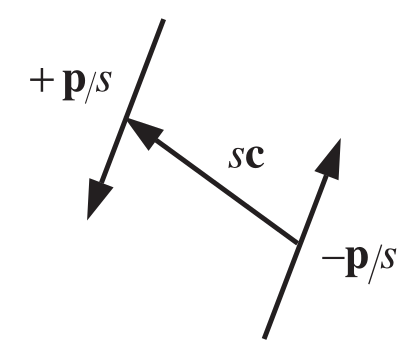
\includegraphics[width=0.5\linewidth]{4p10.png}
\end{center}

\column{0.55\textwidth}

\begin{alertblock}{Ideia}
Os dipolos possuem orientações opostas:
\[
+\frac{\mathbf p}{s}
\qquad\text{e}\qquad
-\frac{\mathbf p}{s}
\]
separados por:
\[
s\mathbf c.
\]
\end{alertblock}

\begin{mybox}{Resultado}
No limite:
\[
s\to0,
\]
surge um quadrupolo pontual.
\end{mybox}

\end{columns}

\end{frame}

%------------------------------------------------
\begin{frame}{Potencial do Quadrupolo Pontual}

\begin{eqbox}
\begin{equation}
\varphi(\mathbf r)
=
\frac{1}{4\pi\epsilon_0}
(\mathbf c\cdot\nabla)
(\mathbf p\cdot\nabla)
\frac1r
\tag{4.54}
\end{equation}
\end{eqbox}

\begin{mybox}{Interpretação}
O quadrupolo envolve duas derivadas espaciais do potencial:
\[
\frac1r.
\]
\end{mybox}

\notas{pag. 36-37}
\end{frame}

\begin{frame}

\begin{alertblock}{Analogia Multipolar}
\[
\begin{aligned}
\text{monopolo}
&\sim
\frac1r
\\
\text{dipolo}
&\sim
\nabla\frac1r
\\
\text{quadrupolo}
&\sim
\nabla\nabla\frac1r
\end{aligned}
\]
\end{alertblock}

\end{frame}

%------------------------------------------------
\begin{frame}{Forma do Tensor de Quadrupolo}

\begin{eqbox}
\begin{equation}
Q_{ij}
=
\frac12
(c_i p_j+c_j p_i)
\tag{4.55}
\end{equation}
\end{eqbox}

\begin{mybox}{Simetria}
\[
Q_{ij}=Q_{ji}
\]
\end{mybox}

\begin{alertblock}{Consequência}
Uma matriz \(3\times3\) simétrica possui apenas:
\[
6
\]
componentes independentes.
\end{alertblock}

\begin{eqbox}
\begin{equation}
\mathbf Q=
\begin{bmatrix}
Q_{xx} & Q_{xy} & Q_{xz}
\\
Q_{xy} & Q_{yy} & Q_{yz}
\\
Q_{xz} & Q_{yz} & Q_{zz}
\end{bmatrix}
\tag{4.57}
\end{equation}
\end{eqbox}
\notas{pag. 38-39}
\end{frame}

%------------------------------------------------
\begin{frame}{Densidade Singular do Quadrupolo}

\begin{mybox}{Quadrupolo Pontual}
A densidade de carga singular correspondente é:
\end{mybox}

\begin{eqbox}
\begin{equation}
\rho_Q(\mathbf r)
=
Q_{ij}
\nabla_i\nabla_j
\delta(\mathbf r)
\tag{4.56}
\end{equation}
\end{eqbox}
\notas{pag. 40-41}
\end{frame}

\begin{frame}
\begin{alertblock}{Cada Multipolo corresponde a uma derivada adicional da delta}
\begin{itemize}
\item monopolo:
\[
\delta(\mathbf r)
\]
\item dipolo:
\[
\nabla\delta(\mathbf r)
\]
\item quadrupolo:
\[
\nabla\nabla\delta(\mathbf r)
\]
\end{itemize}
\end{alertblock}

\end{frame}

%------------------------------------------------
%================================================
\begin{frame}{O Tensor de Quadrupolo}

\begin{columns}[T]

%-----------------------------------
\column{0.48\textwidth}

\begin{mybox}{Tensor Simétrico}
O tensor de quadrupolo possui a propriedade:
\[
Q_{ij}=Q_{ji}.
\]
\end{mybox}

\vspace{0.2cm}

\begin{eqbox}
\begin{equation}
\mathbf Q=
\begin{bmatrix}
Q_{xx} & Q_{xy} & Q_{xz}
\\
Q_{xy} & Q_{yy} & Q_{yz}
\\
Q_{xz} & Q_{yz} & Q_{zz}
\end{bmatrix}
\tag{4.57}
\end{equation}
\end{eqbox}

%-----------------------------------
\column{0.52\textwidth}

\begin{alertblock}{Consequência}
Uma matriz \(3\times3\) genérica possui:
\[
9
\]
componentes independentes.
\end{alertblock}

\vspace{0.2cm}

\begin{mybox}{Mas a Simetria Impõe}
\[
Q_{xy}=Q_{yx},
\]
\[
Q_{xz}=Q_{zx},
\]
\[
Q_{yz}=Q_{zy}.
\]
\end{mybox}

\vspace{0.3cm}

\begin{center}

\Huge
\[
9-3=6
\]

\vspace{0.2cm}

\Large
Restam apenas:
\[
6
\]
componentes independentes.

\end{center}

\end{columns}

\end{frame}

%================================================
\begin{frame}{Por Que o Tensor é Simétrico?}

\begin{eqbox}
\begin{equation}
Q_{ij}
=
\frac12
\int d^3r\,
\rho(\mathbf r)\,
r_i r_j
\tag{4.53 revisitada}
\end{equation}
\end{eqbox}

\begin{mybox}{Observe}
Os fatores:
\[
r_i r_j
\]
satisfazem:
\[
r_i r_j=r_j r_i.
\]
\end{mybox}

\begin{alertblock}{Exemplo}
\[
xy=yx,
\qquad
xz=zx.
\]
\end{alertblock}

\begin{center}

Portanto:
\[
Q_{ij}=Q_{ji}.
\]

O tensor já nasce naturalmente simétrico.

\end{center}

\end{frame}

%================================================

\begin{frame}{Sistema de Eixos Principais}

\begin{columns}[T]

%-----------------------------------
\column{0.48\textwidth}

\begin{mybox}{Ideia Física}
Existe um sistema especial de coordenadas:
\[
(x',y',z')
\]
em que o tensor de quadrupolo fica diagonal.
\end{mybox}

\vspace{0.2cm}

\begin{eqbox}
\begin{equation}
\mathbf Q'=
\begin{bmatrix}
Q'_{xx} & 0 & 0
\\
0 & Q'_{yy} & 0
\\
0 & 0 & Q'_{zz}
\end{bmatrix}
\end{equation}
\end{eqbox}

%-----------------------------------
\column{0.52\textwidth}

\begin{alertblock}{Significado}
Nesse sistema:
\begin{itemize}
\item desaparecem os termos mistos;

\vspace{0.15cm}

\item a geometria da distribuição fica mais clara;

\vspace{0.15cm}

\item os eixos se alinham às direções naturais da distribuição.
\end{itemize}
\end{alertblock}

\vspace{0.3cm}

\begin{center}

\Large
Tensor original:
\[
\mathbf Q
\]

\vspace{0.2cm}

\Large
\(\Downarrow\)

\vspace{0.2cm}

\Large
Mudança de base

\vspace{0.2cm}

\Large
\(\Downarrow\)

\vspace{0.2cm}

\Large
Tensor diagonal:
\[
\mathbf Q'
\]

\end{center}

\end{columns}

\end{frame}


%================================================
\begin{frame}{Interpretação dos Termos Mistos}

\begin{columns}

\column{0.5\textwidth}

\begin{mybox}{Termos Diagonais}
\[
Q_{xx},
\quad
Q_{yy},
\quad
Q_{zz}
\]
medem alongamentos ao longo dos eixos principais.
\end{mybox}

\column{0.5\textwidth}

\begin{alertblock}{Termos Mistos}
\[
Q_{xy},
\quad
Q_{xz},
\quad
Q_{yz}
\]
medem inclinações e correlações geométricas entre direções espaciais.
\end{alertblock}

\end{columns}

\vspace{0.5cm}

\begin{center}

\Large
Diagonalizar o tensor significa remover essas correlações.

\end{center}

\end{frame}

%================================================

\begin{frame}{Definição no Sistema Principal}

\begin{columns}[T]

%-----------------------------------
\column{0.52\textwidth}

\begin{eqbox}
\begin{equation}
Q'_{ij}
=
\frac12
\delta_{ij}
\int d^3r'\,
\rho(\mathbf r')\,
r'_i r'_j
\tag{4.58}
\end{equation}
\end{eqbox}

\vspace{0.2cm}

\begin{mybox}{Papel da Delta de Kronecker}
\[
\delta_{ij}
=
\begin{cases}
1 & i=j
\\
0 & i\neq j
\end{cases}
\]
\end{mybox}

%-----------------------------------
\column{0.48\textwidth}

\begin{alertblock}{Consequência}
A delta elimina automaticamente:
\[
Q'_{xy},
\]
\[
Q'_{xz},
\]
\[
Q'_{yz}.
\]
\end{alertblock}


\begin{center}


Somente os termos:

\[
Q'_{xx},
\qquad
Q'_{yy},
\qquad
Q'_{zz}
\]


sobrevivem.

\end{center}

\vspace{0.3cm}

\begin{mybox}{Interpretação}
No sistema principal,
o tensor fica completamente diagonal.
\end{mybox}

\end{columns}

\end{frame}


%================================================

%================================================
\begin{frame}{Diagonalização e Álgebra Linear}

\begin{mybox}{Transformação de Base}
A mudança de coordenadas é escrita como:
\end{mybox}

\begin{eqbox}
\begin{equation}
\mathbf Q'
=
\mathbf U^{-1}
\mathbf Q
\mathbf U
\tag{4.59}
\end{equation}
\end{eqbox}

\begin{mybox}{Quem é \(\mathbf U\)?}
\[
\mathbf U
\]
é a matriz formada pelos autovetores de:
\[
\mathbf Q.
\]
\end{mybox}

\end{frame}

%================================================
\begin{frame}{Diagonalização: Resultado Físico}

\begin{alertblock}{Resultado Importante}
Toda matriz simétrica:
\[
Q_{ij}=Q_{ji}
\]
pode ser diagonalizada.
\end{alertblock}

\begin{center}
\Large
\[
\mathbf Q
\quad
\Longrightarrow
\quad
\mathbf Q'
=
\begin{bmatrix}
Q'_{xx} & 0 & 0
\\
0 & Q'_{yy} & 0
\\
0 & 0 & Q'_{zz}
\end{bmatrix}
\]
\end{center}

\begin{mybox}{Interpretação}
A nova base revela os eixos principais da distribuição de carga.
\end{mybox}

\end{frame}


%================================================
\begin{frame}{Autovalores e Autovetores}

\begin{columns}

\column{0.5\textwidth}

\begin{mybox}{Autovetores}
Definem as direções principais da distribuição de carga.
\end{mybox}

\vspace{0.3cm}

\begin{eqbox}
\[
\mathbf Q\mathbf v
=
\lambda \mathbf v
\]
\end{eqbox}

\column{0.5\textwidth}

\begin{alertblock}{Autovalores}
Os números:
\[
Q'_{xx},
\quad
Q'_{yy},
\quad
Q'_{zz}
\]
são os autovalores do tensor.
\end{alertblock}

\end{columns}

\vspace{0.5cm}

\begin{center}

\Large
Eles quantificam a deformação espacial ao longo dos eixos principais.

\end{center}

\end{frame}

%================================================
\begin{frame}{Analogia com o Tensor de Inércia}

\begin{mybox}{Observação Importante do Livro}
O tensor de quadrupolo é matematicamente análogo ao tensor de inércia da mecânica clássica.
\end{mybox}

\begin{columns}

\column{0.48\textwidth}

\begin{alertblock}{Tensor de Quadrupolo}
Descreve:
\begin{itemize}
\item geometria da distribuição de carga;
\item deformações elétricas;
\item anisotropias do potencial.
\end{itemize}
\end{alertblock}

\column{0.48\textwidth}

\begin{alertblock}{Tensor de Inércia}
Descreve:
\begin{itemize}
\item distribuição de massa;
\item resistência à rotação;
\item eixos principais do corpo.
\end{itemize}
\end{alertblock}

\end{columns}

\vspace{0.4cm}

\begin{center}

\Large
Ambos são tensores simétricos diagonalizáveis.

\end{center}

\end{frame}

%================================================
\begin{frame}{Resumo Conceitual}

\begin{center}

\Huge
O Quadrupolo Elétrico

\vspace{0.4cm}

mede deformações espaciais da distribuição de carga.

\end{center}

\vspace{0.5cm}

\begin{itemize}
\item Tensor simétrico:
\[
Q_{ij}=Q_{ji}
\]

\item Apenas 6 componentes independentes;

\item Pode ser diagonalizado;

\item Possui eixos principais naturais;

\item É análogo ao tensor de inércia.
\end{itemize}

\end{frame}


%================================================


\begin{frame}{Tensor de Quadrupolo Sem Traço}

\begin{mybox}{Motivação}
Nem sempre é conveniente medir ou escrever o tensor de quadrupolo no sistema de eixos principais.
\end{mybox}

\vspace{0.3cm}

\begin{alertblock}{Problema}
Em um sistema arbitrário, o tensor primitivo:
\[
Q_{ij}
=
\frac12
\int d^3r'\,
\rho(\mathbf r')r'_i r'_j
\]
possui:
\[
6
\]
componentes independentes.
\end{alertblock}

\vspace{0.3cm}

\begin{center}
\Large
\[
Q_{ij}
\]
\end{center}

\end{frame}

%-------------------------------------------------

\begin{frame}{Tensor de Quadrupolo Sem Traço}

\begin{columns}[T]

%-----------------------------------
\column{0.50\textwidth}

\small

\begin{mybox}{Estratégia}
Podemos reescrever o potencial usando um novo tensor:
\[
\Theta_{ij},
\]
que é:
\begin{itemize}
\item simétrico;
\item sem traço;
\item mais econômico.
\end{itemize}
\end{mybox}

%-----------------------------------
\column{0.50\textwidth}

\begin{center}

\Large
\[
Q_{ij}
\quad
\Longrightarrow
\quad
\Theta_{ij}
\]

\vspace{0.5cm}

\Large
\[
6
\quad\longrightarrow\quad
5
\]

\vspace{0.2cm}

componentes independentes

\end{center}

\end{columns}

\end{frame}




%================================================
\begin{frame}{Substituindo \(Q_{ij}\) no Potencial}

\begin{mybox}{Potencial quadrupolar}
Começamos de:
\[
\varphi(\mathbf r)
=
\frac{1}{4\pi\epsilon_0}
Q_{ij}
\frac{3r_i r_j-\delta_{ij}r^2}{r^5}.
\]
\end{mybox}

Usando:

\[
Q_{ij}
=
\frac12
\int d^3r'\,
\rho(\mathbf r')r'_i r'_j,
\]

obtemos:

\begin{eqbox}
\begin{equation}
\varphi(\mathbf r)
=
\frac{1}{4\pi\epsilon_0}
\left\{
\frac12
\int d^3r'\,
\rho(\mathbf r')r'_i r'_j
\right\}
\frac{3r_i r_j-r^2\delta_{ij}}{r^5}.
\tag{4.60}
\end{equation}
\end{eqbox}

\end{frame}

%================================================
\begin{frame}{A Identidade Algébrica Importante}

\begin{mybox}{Identidade usada}
O passo central é usar:
\end{mybox}

\begin{eqbox}
\begin{equation}
r'_i r'_j r^2\delta_{ij}
=
r^2r'^2
=
r_i r_j r'^2\delta_{ij}.
\tag{4.61}
\end{equation}
\end{eqbox}

\begin{alertblock}{Por quê?}
Como há soma sobre \(i\) e \(j\), temos:
\[
r'_i r'_j\delta_{ij}
=
r'_i r'_i
=
r'^2.
\]
Logo:
\[
r'_i r'_j r^2\delta_{ij}
=
r^2 r'^2.
\]
\end{alertblock}

\end{frame}

%================================================
\begin{frame}{Reorganizando o Numerador}

A Eq. (4.60) contém o produto:

\[
r'_i r'_j
\left(
3r_i r_j-r^2\delta_{ij}
\right).
\]

Distribuindo:

\[
3r'_i r'_j r_i r_j
-
r'_i r'_j r^2\delta_{ij}.
\]

Agora usamos a identidade:

\[
r'_i r'_j r^2\delta_{ij}
=
r_i r_j r'^2\delta_{ij}.
\]

Portanto:

\[
3r'_i r'_j r_i r_j
-
r_i r_j r'^2\delta_{ij}
=
\left(
3r'_i r'_j
-
r'^2\delta_{ij}
\right)
r_i r_j.
\]

\end{frame}

%================================================
\begin{frame}{Nova Forma do Potencial}

Assim, a Eq. (4.60) pode ser escrita como:

\begin{eqbox}
\begin{equation}
\varphi(\mathbf r)
=
\frac{1}{4\pi\epsilon_0}
\left\{
\frac12
\int d^3r'\,
\rho(\mathbf r')
\left(
3r'_i r'_j-r'^2\delta_{ij}
\right)
\right\}
\frac{r_i r_j}{r^5}.
\tag{4.62}
\end{equation}
\end{eqbox}

\begin{mybox}{Ideia}
Toda a informação da distribuição de carga agora está dentro das chaves.
\end{mybox}

\begin{alertblock}{Próximo passo}
Definimos essa quantidade como um novo tensor:
\[
\Theta_{ij}.
\]
\end{alertblock}
\notas{pag. 42-44}

\end{frame}

%================================================
\begin{frame}{Definição do Tensor Sem Traço}

\begin{eqbox}
\begin{equation}
\Theta_{ij}
=
\frac12
\int d^3r'\,
\rho(\mathbf r')
\left(
3r'_i r'_j-r'^2\delta_{ij}
\right)
=
3Q_{ij}-Q_{kk}\delta_{ij}.
\tag{4.63}
\end{equation}
\end{eqbox}

\begin{mybox}{Comparação}
O tensor primitivo era:
\[
Q_{ij}
=
\frac12
\int d^3r'\,
\rho(\mathbf r')r'_i r'_j.
\]
\end{mybox}

\begin{alertblock}{O que mudou?}
Subtraímos a parte proporcional a:
\[
\delta_{ij}.
\]
Essa parte corresponde ao traço, isto é, à parte esfericamente simétrica.
\end{alertblock}

\end{frame}

%================================================
\begin{frame}{Potencial com \(\Theta_{ij}\)}

Com a definição:

\[
\Theta_{ij}
=
\frac12
\int d^3r'\,
\rho(\mathbf r')
\left(
3r'_i r'_j-r'^2\delta_{ij}
\right),
\]

a Eq. (4.62) fica:

\begin{eqbox}
\begin{equation}
\varphi(\mathbf r)
=
\frac{1}{4\pi\epsilon_0}
\Theta_{ij}
\frac{r_i r_j}{r^5}.
\tag{4.64}
\end{equation}
\end{eqbox}

\begin{mybox}{Vantagem}
O potencial fica mais simples:
\[
\text{tensor}
\times
\text{geometria angular}.
\]
\end{mybox}
\end{frame}

%================================================
\begin{frame}{Por Que ``Sem Traço''?}

\begin{mybox}{Traço de um tensor}
O traço é a soma dos elementos diagonais:
\[
\mathrm{Tr}[\boldsymbol{\Theta}]
=
\Theta_{xx}+\Theta_{yy}+\Theta_{zz}.
\]
\end{mybox}

Em notação indicial:

\[
\mathrm{Tr}[\boldsymbol{\Theta}]
=
\delta_{ij}\Theta_{ij}.
\]

Usando a definição de \(\Theta_{ij}\):

\begin{eqbox}
\begin{equation}
\mathrm{Tr}[\boldsymbol{\Theta}]
=
\delta_{ij}\Theta_{ij}
=
\frac12
\int d^3r\,
\rho(\mathbf r)
\left(
3r_i r_i-r^2\delta_{ii}
\right).
\tag{4.65}
\end{equation}
\end{eqbox}

\end{frame}

%================================================
\begin{frame}{Mostrando que o Traço é Zero}

Agora usamos:

\[
r_i r_i
=
r^2
\]

e, em três dimensões,

\[
\delta_{ii}
=
\delta_{xx}+\delta_{yy}+\delta_{zz}
=
3.
\]

Logo:

\[
3r_i r_i-r^2\delta_{ii}
=
3r^2-3r^2
=
0.
\]

Portanto:

\begin{eqbox}
\begin{equation}
\mathrm{Tr}[\boldsymbol{\Theta}]
=
0.
\tag{4.65}
\end{equation}
\end{eqbox}



\end{frame}

%================================================
\begin{frame}{Restrição Sobre as Componentes}

Como o traço é zero:

\begin{eqbox}
\begin{equation}
\mathrm{Tr}[\boldsymbol{\Theta}]
=
\Theta_{xx}
+
\Theta_{yy}
+
\Theta_{zz}
=
0.
\tag{4.66}
\end{equation}
\end{eqbox}

\begin{alertblock}{Consequência}
As três componentes diagonais não são independentes.
\end{alertblock}

Por exemplo:

\[
\Theta_{zz}
=
-\Theta_{xx}-\Theta_{yy}.
\]

\begin{center}
\Large
Assim, o número de componentes independentes cai de:
\[
6
\quad\longrightarrow\quad
5.
\]
\end{center}

\end{frame}

%================================================
\begin{frame}{Por Que Isso é Mais Econômico?}

\begin{columns}[T]

\column{0.48\textwidth}

\begin{mybox}{Tensor primitivo}
\[
Q_{ij}=Q_{ji}
\]
possui:
\[
6
\]
componentes independentes.
\end{mybox}

\column{0.48\textwidth}

\begin{alertblock}{Tensor sem traço}
\[
\Theta_{ij}=\Theta_{ji},
\qquad
\mathrm{Tr}[\Theta]=0
\]
possui:
\[
5
\]
componentes independentes.
\end{alertblock}

\end{columns}

\vspace{0.5cm}

\begin{center}
\Large
O tensor sem traço remove a parte esfericamente simétrica, que não contribui de forma independente para o potencial quadrupolar.
\end{center}

\end{frame}

%================================================
\begin{frame}{Resumo Conceitual}

\begin{columns}[T]

%-----------------------------------
\column{0.52\textwidth}

\begin{mybox}{Mensagem Principal}
O tensor de quadrupolo sem traço é definido por:
\[
\Theta_{ij}
=
3Q_{ij}
-
Q_{kk}\delta_{ij}.
\]
\end{mybox}

\vspace{0.2cm}

\begin{eqbox}
\[
\varphi(\mathbf r)
=
\frac{1}{4\pi\epsilon_0}
\Theta_{ij}
\frac{r_i r_j}{r^5}.
\]
\end{eqbox}

%-----------------------------------
\column{0.48\textwidth}

\begin{alertblock}{Por que ele é útil?}
\begin{itemize}
\item simplifica o potencial;

\vspace{0.1cm}

\item funciona em coordenadas arbitrárias;

\vspace{0.1cm}

\item reduz o número de componentes independentes;

\vspace{0.1cm}

\item separa a parte verdadeiramente quadrupolar da parte esférica.
\end{itemize}
\end{alertblock}

\vspace{0.3cm}

\begin{center}


\[
Q_{ij}
\quad\Rightarrow\quad
\Theta_{ij}
\]



\Large
\[
6
\quad\longrightarrow\quad
5
\]



componentes independentes

\end{center}

\end{columns}

\end{frame}



%====================================================
\section{Momentos de Quadrupolo Nuclear}
%====================================================

%----------------------------------------------------
\begin{frame}{Aplicação: Momentos de Quadrupolo Nuclear}

\begin{mybox}{Ideia Física}
O tensor de quadrupolo mede desvios da simetria esférica
em distribuições de carga.
\end{mybox}

\vspace{0.3cm}

\begin{alertblock}{Núcleos Atômicos}
Muitos núcleos possuem simetria de rotação em torno de um eixo principal,
geralmente escolhido como o eixo \(z\).
\end{alertblock}

\end{frame}

\begin{frame}

Se o núcleo é axialmente simétrico:

\[
\Theta_{xx}=\Theta_{yy}.
\]

Além disso, como o tensor é sem traço:

\[
\Theta_{xx}+\Theta_{yy}+\Theta_{zz}=0.
\]

Substituindo a simetria axial:

\[
2\Theta_{xx}+\Theta_{zz}=0.
\]

Portanto:

\begin{eqbox}
\begin{equation}
\Theta_{zz}
=
-2\Theta_{xx}
=
-2\Theta_{yy}
\tag{4.70}
\end{equation}
\end{eqbox}

\end{frame}

%----------------------------------------------------
\begin{frame}{Apenas Um Parâmetro Independente}

\begin{mybox}{Consequência}
Devido à simetria axial e à condição de traço nulo,
todo o tensor pode ser descrito por apenas:
\[
Q\equiv \Theta_{zz}.
\]
\end{mybox}

\vspace{0.4cm}

\begin{center}

\Large
\[
\Theta_{ij}
\Longrightarrow
Q
\]

\end{center}

\vspace{0.3cm}

\begin{alertblock}{Interpretação}
O sinal de \(Q\) revela o formato da distribuição de carga nuclear.
\end{alertblock}

\end{frame}

%----------------------------------------------------
\begin{frame}{Interpretação Geométrica do Quadrupolo}

\begin{columns}[T]

%---------------------------------
\column{0.55\textwidth}

\small

\begin{mybox}{Caso Esférico}
Se:
\[
Q=0,
\]
a distribuição é aproximadamente esférica.
\end{mybox}

\vspace{0.2cm}

\begin{mybox}{Caso Prolato}
Se:
\[
Q>0,
\]
o núcleo é alongado ao longo do eixo \(z\),
como um charuto.
\end{mybox}




%---------------------------------
\column{0.45\textwidth}
\begin{mybox}{Caso Oblato}
Se:
\[
Q<0,
\]
o núcleo é achatado ao longo do eixo \(z\),
como uma abóbora.
\end{mybox}

\begin{center}
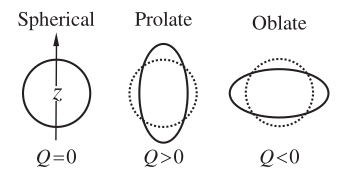
\includegraphics[width=0.6\linewidth]{4p11.png}
\end{center}

\end{columns}

\end{frame}

%----------------------------------------------------
\begin{frame}{Por Que o Sinal de \(Q\) Define a Forma?}

\small

Lembre que:

\begin{eqbox}
\begin{equation}
\Theta_{zz}
=
\frac12
\int d^3r'\,
\rho(\mathbf r')
\left(
3z'^2-r'^2
\right)
\tag{4.63}
\end{equation}
\end{eqbox}

\vspace{0.2cm}

\begin{itemize}

\item Se a carga se concentra ao longo do eixo \(z\),
então:
\[
z'^2
\]
tende a dominar.

\item Nesse caso:
\[
3z'^2-r'^2>0,
\]
e o momento quadrupolar fica positivo.

\item Isso produz um núcleo alongado:
\[
Q>0.
\]

\end{itemize}

\end{frame}

\begin{frame}

\begin{alertblock}{Já para núcleos achatados}
Grande parte da carga fica distribuída no plano transversal,
fazendo:
\[
r'^2 > 3z'^2
\]
em média, o que leva a:
\[
Q<0.
\]
\end{alertblock}

\end{frame}

%----------------------------------------------------
\begin{frame}{Dados Experimentais de Quadrupolo Nuclear}

\begin{center}
\begin{figure}
    \centering

    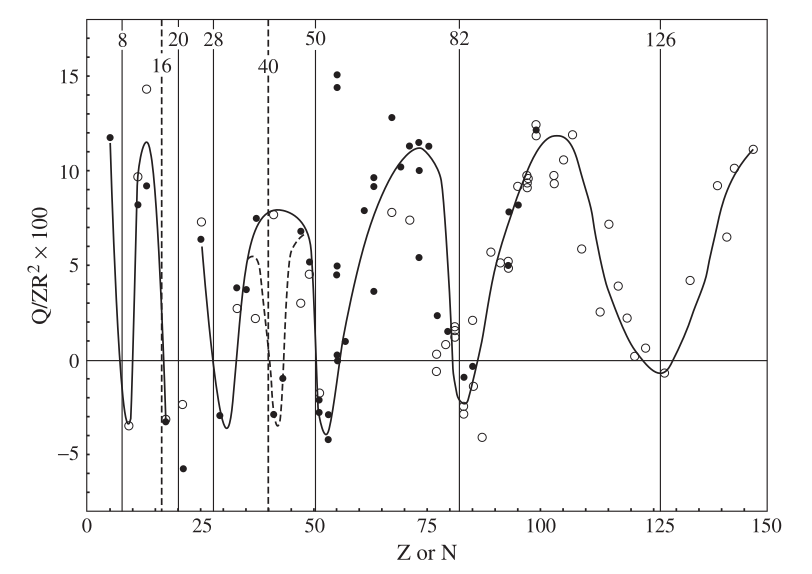
\includegraphics[width=0.5\linewidth]{4p12.png}

    \vspace{-0.2cm}

    {\fontsize{4.5pt}{5pt}\selectfont
    \caption{
    Parâmetro de quadrupolo elétrico do estado fundamental \(Q\) para núcleos de massa ímpar. Os círculos preenchidos (abertos) representam núcleos com número ímpar de prótons (nêutrons) \(Z(N)\). Os dados foram normalizados por \(ZR^2\), onde \(R\) é o raio nuclear. As linhas verticais indicam os números “mágicos”, nos quais camadas ou subcamadas nucleares se fecham. 
    }
    }

\end{figure}
\end{center}

\end{frame}

%----------------------------------------------------
\begin{frame}{Interpretando o Gráfico Experimental}

\small

\begin{columns}[T]

%---------------------------------
\column{0.50\textwidth}

\begin{mybox}{Eixos do gráfico}
\[
Q/ZR^2
\]
mede o quadrupolo elétrico normalizado.

\vspace{0.2cm}

O eixo horizontal representa:
\[
Z \ \text{ou}\ N,
\]
isto é:

\begin{itemize}
\item número de prótons;
\item ou número de nêutrons.
\end{itemize}
\end{mybox}

%---------------------------------
\column{0.50\textwidth}

\begin{alertblock}{Linhas verticais}
As linhas verticais indicam
os chamados:
\[
\textit{magic numbers}.
\]

Eles correspondem ao fechamento de camadas nucleares.
\end{alertblock}
\begin{mybox}{Resultado Importante}
Quando uma camada fecha:
\[
Q\approx0,
\]
pois o núcleo tende a recuperar simetria esférica.
\end{mybox}
\end{columns}





\end{frame}

%----------------------------------------------------
\begin{frame}{Números Mágicos}

\begin{center}

\Large
\[
2,\ 8,\ 20,\ 28,\ 50,\ 82,\ 126
\]

\end{center}

\vspace{0.4cm}

\begin{mybox}{Interpretação}
Esses números aparecem naturalmente no modelo de camadas nucleares.
Eles correspondem a níveis nucleares completamente preenchidos.
\end{mybox}

\vspace{0.3cm}

\begin{alertblock}{Analogia}
São análogos aos gases nobres na estrutura eletrônica atômica:
camadas completas tendem a produzir sistemas mais estáveis e mais simétricos.
\end{alertblock}

\end{frame}

%----------------------------------------------------
\begin{frame}{Predominância de Núcleos Prolatos}

\small

Os dados experimentais mostram algo curioso:

\begin{center}

\Large
núcleos prolatos aparecem com maior frequência.

\end{center}

\vspace{0.3cm}

\begin{mybox}{Observação Experimental}
Após o fechamento de uma camada nuclear,
muitos núcleos tornam-se inicialmente:
\[
Q<0
\]
(oblatos),
mas rapidamente passam para:
\[
Q>0
\]
(prolatos).
\end{mybox}

\end{frame}

\begin{frame}

\begin{alertblock}{Questão em Aberto}
Ainda não existe uma explicação simples e definitiva
para a predominância observada de formas prolatas na natureza.
\end{alertblock}

\end{frame}

%====================================================
\section{Exemplo: Elipsoide Uniformemente Carregado}
%====================================================

%----------------------------------------------------
\begin{frame}{Exemplo 4.2: Elipsoide Uniforme}

\begin{columns}[T]

%-----------------------------------
\column{0.52\textwidth}

\small

\begin{mybox}{Problema}
Calcular o tensor de quadrupolo sem traço
\[
\Theta_{ij}
\]
para um elipsoide com:

\begin{itemize}
\item densidade uniforme \(\rho\);
\item volume \(V\);
\item semi-eixos \(a_x,a_y,a_z\).
\end{itemize}

O centro do elipsoide é escolhido como origem.
\end{mybox}

%-----------------------------------
\column{0.48\textwidth}

\small

A superfície do elipsoide é:

\begin{eqbox}
\begin{equation}
\frac{x'^2}{a_x^2}
+
\frac{y'^2}{a_y^2}
+
\frac{z'^2}{a_z^2}
=
1
\tag{4.71}
\end{equation}
\end{eqbox}

\vspace{0.4cm}

\begin{center}

\Large
Elipsoide

\vspace{0.2cm}

\[
a_x,\ a_y,\ a_z
\]

\end{center}

\end{columns}

\end{frame}

\begin{frame}{Elipsoide}
    \begin{figure}
        \centering
        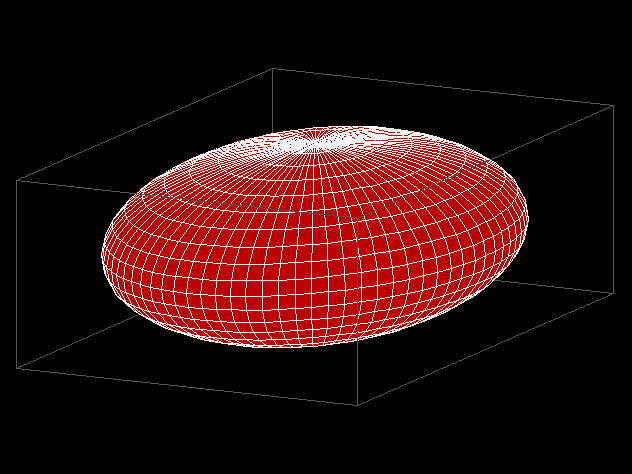
\includegraphics[width=0.5\linewidth]{elipsoide.png}

    \end{figure}
\end{frame}
%----------------------------------------------------
\begin{frame}{Tensor no Sistema de Eixos Principais}

\small

\begin{mybox}{Simetria}
Como os eixos coordenados coincidem com os eixos principais do elipsoide:

\[
\Theta_{xy}
=
\Theta_{xz}
=
\Theta_{yz}
=
0.
\]
\end{mybox}

\vspace{0.3cm}

Isso ocorre porque integrais contendo termos ímpares,
como:
\[
xy,\ xz,\ yz,
\]
cancelam-se pela simetria do volume.
 
\vspace{0.3cm}

Assim, basta calcular os elementos diagonais.

Por exemplo:

\begin{eqbox}
\begin{equation}
\Theta_{xx}
=
\frac12
\rho
\int_V d^3r'
\left(
3x'^2-r'^2
\right)
\tag{4.72}
\end{equation}
\end{eqbox}

Como:
\[
r'^2=x'^2+y'^2+z'^2,
\]
temos:

\[
3x'^2-r'^2
=
2x'^2-y'^2-z'^2.
\]

\end{frame}


%----------------------------------------------------
\begin{frame}{Mudança de Variáveis}

\small

Definimos novas coordenadas adimensionais:

\begin{eqbox}
\begin{equation}
x'=a_x x,
\qquad
y'=a_y y,
\qquad
z'=a_z z.
\tag{4.73}
\end{equation}
\end{eqbox}

Substituindo na equação do elipsoide:

\[
\frac{(a_xx)^2}{a_x^2}
+
\frac{(a_yy)^2}{a_y^2}
+
\frac{(a_zz)^2}{a_z^2}
=
1,
\]

obtemos:

\[
x^2+y^2+z^2=1.
\]

\vspace{0.3cm}

\begin{alertblock}{Resultado Importante}
A integral sobre o elipsoide transforma-se
em uma integral sobre uma esfera unitária.
\end{alertblock}

\end{frame}

%----------------------------------------------------
\begin{frame}{Jacobiano da Transformação}

\small

O elemento de volume transforma-se como:

\[
d^3r'
=
dx'\,dy'\,dz'.
\]

Usando:

\[
dx'=a_xdx,
\qquad
dy'=a_ydy,
\qquad
dz'=a_zdz,
\]

segue que:

\begin{eqbox}
\begin{equation}
d^3r'
=
a_xa_ya_z\,d^3r.
\tag{4.74}
\end{equation}
\end{eqbox}

Substituindo tudo em \(\Theta_{xx}\):

\[
\Theta_{xx}
=
\frac12
\rho a_xa_ya_z
\int d^3r
\left(
2a_x^2x^2
-
a_y^2y^2
-
a_z^2z^2
\right).
\]

\end{frame}

%----------------------------------------------------
\begin{frame}{Integrais na Esfera Unitária}

\small

Pela simetria esférica:

\[
\int d^3r\,x^2
=
\int d^3r\,y^2
=
\int d^3r\,z^2.
\]

Além disso:

\[
x^2+y^2+z^2=r^2.
\]

Somando as três integrais:

\[
3
\int d^3r\,x^2
=
\int d^3r\,r^2.
\]

Portanto:

\begin{eqbox}
\begin{equation}
\int d^3r\,x^2
=
\frac13
\int d^3r\,r^2.
\tag{4.75}
\end{equation}
\end{eqbox}

\end{frame}

%----------------------------------------------------
\begin{frame}{Calculando a Integral Radial}

\small

Na esfera unitária:

\[
d^3r
=
r^2\sin\theta\,dr\,d\theta\,d\phi.
\]

Então:

\[
\int d^3r\,r^2
=
\int_0^1dr\,r^4
\int_0^\pi d\theta\,\sin\theta
\int_0^{2\pi}d\phi.
\]

Calculando:

\[
\int_0^\pi\sin\theta\,d\theta=2,
\]

\[
\int_0^{2\pi}d\phi=2\pi,
\]

\[
\int_0^1 r^4dr=\frac15.
\]

Logo:

\[
\int d^3r\,r^2
=
\frac{4\pi}{5}.
\]

Portanto:

\begin{eqbox}
\begin{equation}
\int d^3r\,x^2
=
\int d^3r\,y^2
=
\int d^3r\,z^2
=
\frac{4\pi}{15}.
\tag{4.76}
\end{equation}
\end{eqbox}

\end{frame}

%----------------------------------------------------
\begin{frame}{Resultado Final para \(\Theta_{xx}\)}

\small

Substituindo as integrais:

\[
\Theta_{xx}
=
\frac12
\rho a_xa_ya_z
\frac{4\pi}{15}
\left(
2a_x^2-a_y^2-a_z^2
\right).
\]

Agora usamos o volume do elipsoide:

\begin{eqbox}
\begin{equation}
V
=
\frac{4\pi}{3}
a_xa_ya_z.
\tag{4.77}
\end{equation}
\end{eqbox}

Assim:

\[
\frac12
\rho a_xa_ya_z
\frac{4\pi}{15}
=
\frac{\rho V}{10}.
\]

Finalmente:

\begin{eqbox}
\begin{equation}
\Theta_{xx}
=
\frac1{10}
\rho V
\left(
2a_x^2-a_y^2-a_z^2
\right).
\tag{4.78}
\end{equation}
\end{eqbox}

\end{frame}

%----------------------------------------------------
\begin{frame}{Outras Componentes}

\small

Por simetria cíclica:

\begin{eqbox}
\begin{align}
\Theta_{yy}
&=
\frac1{10}
\rho V
\left(
2a_y^2-a_z^2-a_x^2
\right),
\tag{4.79}
\\[0.3cm]
\Theta_{zz}
&=
\frac1{10}
\rho V
\left(
2a_z^2-a_x^2-a_y^2
\right).
\tag{4.80}
\end{align}
\end{eqbox}

\vspace{0.3cm}

Somando:

\[
\Theta_{xx}
+
\Theta_{yy}
+
\Theta_{zz}
=
0.
\]

\begin{alertblock}{Verificação}
O tensor é realmente sem traço.
\end{alertblock}

\end{frame}

%----------------------------------------------------
\begin{frame}{Interpretação Física}

\small

\begin{columns}[T]

%--------------------------------
\column{0.5\textwidth}

\begin{mybox}{Elipsoide Alongado}
Se:
\[
a_z>a_x,a_y,
\]
então:
\[
\Theta_{zz}>0.
\]

A distribuição é prolata.
\end{mybox}

%--------------------------------
\column{0.5\textwidth}

\begin{mybox}{Elipsoide Achatado}
Se:
\[
a_z<a_x,a_y,
\]
então:
\[
\Theta_{zz}<0.
\]

A distribuição é oblata.
\end{mybox}

\end{columns}

\vspace{0.5cm}

\begin{center}

\Large
o tensor quadrupolar mede desvios da esfericidade

\end{center}

\end{frame}

\end{document}